\input{glyphtounicode}
\pdfgentounicode=1
% Map minted line-break glyphs to Unicode to satisfy PDF/A
\pdfglyphtounicode{arrowhookleft}{21A9}
\pdfglyphtounicode{arrowhookright}{21AA}
\DocumentMetadata{
    pdfstandard=A-3a,
    pdfversion=1.7,
    lang=it
}

\documentclass[
    table,
    12pt,
    oneside,
    a4paper,
    italian
]{book}

\input{config/packages}
\input{config/thesis_config}

\date{}

\hypersetup{pdfstartview=}
\begin{document}
    \frontmatter
    \input{preface/1_title_page}
    %\increasepagenumbering % increase the page numbrering by 1, in order to cout the frontispiece
    %\input{preface/2_copyright}
    %\cleardoublepage
\phantomsection
\pdfbookmark{Ringraziamenti}{Ringraziamenti}

\begin{flushright}{
    \slshape
    ``It's not a bug, it's a feature.''} \\
    \medskip
    --- Matt Groening, \textit{Futurama}.
\end{flushright}

\begingroup
\let\clearpage\relax
\let\cleardoublepage\relax
\let\cleardoublepage\relax

\chapter*{Ringraziamenti}

\noindent Desidero esprimere la mia gratitudine alla \myProf, mia relatrice, per l'aiuto e il sostegno che mi ha dato durante la stesura dell'elaborato.

\vspace{0.35cm}

\noindent Vorrei anche ringraziare, con affetto, i miei genitori per il loro sostegno, il grande aiuto e la loro presenza in ogni momento durante gli anni di studio.

\vspace{0.35cm}

\noindent Desidero poi ringraziare i miei amici per i bellissimi anni trascorsi insieme e le mille avventure vissute.

\vspace{0.75cm}

\noindent{\myLocation, \myTime}
\hfill \textit{\myName}

\endgroup

    %\cleardoublepage
\phantomsection
\pdfbookmark{Compendio}{Compendio}
\begingroup
\let\clearpage\relax
\let\cleardoublepage\relax
\chapter*{Sommario}

Durante lo stage presso Spazio Dev ho contribuito alla realizzazione di \mbox{ErpAI}, un nuovo ERP modulare. Il lavoro si è concentrato sull’implementazione di un motore di previsione vendite per anticipare la produzione: a partire da uno storico di fatture che descrivono le vendite passate dei prodotti, il modello stima la domanda futura per supportare decisioni operative tempestive e ridurre il rischio di stock-out. La tesi documenta progettazione, scelta delle feature e addestramento del modello XGBoost, selezionato per l’equilibrio tra accuratezza predittiva, tempi di training e impiego in contesti produttivi.

\endgroup
\vfill

    %\input{preface/5_table_of_contents}
    %\printglossary[type=\acronymtype, title=Acronimi e abbreviazioni, toctitle=Acronimi e abbreviazioni]
    %\printglossary[type=main, title=Glossario, toctitle=Glossario]
    %\blankpage % example of a blank page that also increases the page couter by 1

    \mainmatter
    \chapter{Prova}
    Contenuto di test per generare almeno una pagina e produrre un PDF valido.
    %\chapter{Introduzione}
\label{chap:introduzione}

\section{L'azienda}
Spazio Dev S.r.l.\footnote{\url{https://spaziodev.eu/}} è una realtà giovane, fondata nel 2023 a Tombolo (PD), che opera come partner tecnologico per aziende industriali e commerciali con un approccio aperto e flessibile. Offre sviluppo software su misura, integrazione di sistemi e servizi cloud; progetta siti web, e-commerce e soluzioni gestionali per migliorare i processi produttivi e commerciali, con focus su integrazioni affidabili e supporto post-rilascio.
\begin{figure}[H]
    \centering
    
\includegraphics[width=\textwidth]{img/Logo_SpazioDev.png}
    \caption{Logo di Spazio Dev}
    \label{fig:logo-spaziodev}
\end{figure}

\subsection{ErpAI}
\textit{ErpAI} è un progetto di Spazio Dev S.r.l. volto a realizzare un gestionale \acrfull{erp} modulare, destinato a essere venduto e personalizzato per le aziende clienti. La piattaforma è pensata per coprire anagrafiche (prodotti, clienti, fornitori), flussi amministrativi (fatture di vendita e acquisto, ordini, magazzino) e componenti avanzate come schedulazione di macchine/turni e previsione delle vendite. L’architettura modulare consente di attivare solo i domini necessari e di integrarli con sistemi esistenti tramite \acrfull{api}, mantenendo la flessibilità per personalizzazioni settoriali e successive estensioni di prodotto.

\section{L'idea}
Per completare l’offerta di \textit{ErpAI}, è stata identificata la necessità di un motore di previsione vendite che supporti la pianificazione produttiva e riduca il rischio di \textit{stock-out} o \textit{overstock}. Il progetto nasce dal confronto con le richieste di clienti che vogliono decisioni più tempestive su produzione, approvvigionamenti e allocazione delle risorse.

Il lavoro dello stage si concentra su questa componente predittiva: partire dai dati storici delle fatture, pulirli e trasformarli in feature utili, addestrare un modello di \gls{ml} per stimare la domanda futura, valutarlo usando metriche di errore e rendere i risultati disponibili al sistema \acrshort{erp}. Il modulo è implementato in Python ed esposto tramite FastAPI per l’integrazione via \gls{api} con \textit{ErpAI}; include spiegazioni delle previsioni con \gls{shap} per aderire ai principi di \acrfull{xai}. La prima versione è stata sviluppata su un caso aziendale specifico e potrà essere adattata in futuro per gestire dataset e contesti di aziende differenti, variando feature, pre-processing e parametri del modello in base alle esigenze.

\section{Organizzazione del testo}
\begin{description}
    \item[{\hyperref[chap:processi-metodologie]{Il secondo capitolo}}] descrive i processi aziendali e le metodologie adottate durante lo stage.
    \item[{\hyperref[chap:descrizione-stage]{Il terzo capitolo}}] inquadra l’azienda, il percorso di stage e gli obiettivi concordati.
    \item[{\hyperref[chap:analisi-requisiti]{Il quarto capitolo}}] raccoglie e struttura i requisiti funzionali e non funzionali del motore di previsione.
    \item[{\hyperref[chap:design]{Il quinto capitolo}}] illustra la progettazione complessiva: architettura, pipeline dati, modello predittivo e \gls{api} di servizio.
    \item[{\hyperref[chap:codebase]{Il sesto capitolo}}] presenta il codice sviluppato, l’organizzazione dei moduli e gli esempi principali.
    \item[{\hyperref[chap:testing]{Il settimo capitolo}}] documenta la strategia di testing, i test automatici e la pipeline di integrazione continua.
    \item[{\hyperref[chap:conclusioni]{L’ottavo capitolo}}] riporta conclusioni, risultati ottenuti e possibili evoluzioni future.
\end{description}

Per la stesura del testo sono state adottate le seguenti convenzioni tipografiche:
\begin{itemize}
    \item gli acronimi, le abbreviazioni e i termini ambigui o di uso non comune menzionati vengono definiti nel glossario, e questa convenzione è applicata in modo uniforme in tutto il testo;
    \item per la prima occorrenza dei termini riportati nel glossario viene utilizzata la forma estesa seguita dall’acronimo (ad esempio \gls{api});
    \item i termini in lingua straniera o facenti parti del gergo tecnico sono evidenziati con il carattere \textit{corsivo};
    \item i nomi di oggetti, funzioni, tabelle, colonne, classi e rotte \gls{api} sono riportati in carattere \texttt{monospaziato}.
\end{itemize}

\newpage

    %\chapter{Processi aziendali}
\label{chap:processi-metodologie}

\section{Organizzazione e collaborazione}
Lo stage si inserisce nel progetto \textit{ErpAI} di Spazio Dev, con l’obiettivo di realizzare il primo motore di previsione degli acquisti integrato nell’ERP proprietario. Il team conta un referente tecnico aziendale, due sviluppatori e il sottoscritto; lo sviluppo del modulo di previsione e delle componenti di explainable AI è assegnato a me. Le procedure sono in evoluzione perché l’azienda è giovane e in crescita, ma già orientate a documentazione condivisa, verifiche automatizzate e tracciabilità delle decisioni.

\subsection{Ambienti e strumenti di sviluppo}
L’azienda consente a ciascun sviluppatore di utilizzare il proprio sistema operativo e l’IDE preferito, nel rispetto delle convenzioni di progetto. La coerenza tra i team è garantita dalla containerizzazione: tutti i progetti sono eseguiti in Docker e, quando serve un ambiente di sviluppo replicabile, viene adottato ddev. Quest’ultimo offre configurazioni preimpostate e comandi uniformi per avviare i servizi, aggiornare le dipendenze e verificare l’applicazione in locale. Ne derivano onboarding più rapido, dipendenze allineate e test eseguiti in ambienti equivalenti a quelli usati per l’integrazione continua.

\subsection{Modello di lavoro agile}
Il framework adottato è Scrum\footnote{\url{https://it.wikipedia.org/wiki/Scrum_(informatica)}}, che articola il lavoro in iterazioni brevi con fasi di pianificazione, sviluppo, revisione e retrospettiva. I titolari di Spazio Dev esercitano il ruolo di Product Owner definendo priorità, obiettivi di Sprint e criteri di accettazione, e quello di Scrum Master coordinando le cerimonie e rimuovendo gli impedimenti. Gli sviluppatori, incluso il sottoscritto, realizzano le attività di backlog, rendicontano gli avanzamenti e presentano gli incrementi. Ogni Sprint settimanale si apre con la definizione del lavoro da eseguire per \textit{ErpAI} e si chiude con la verifica degli incrementi consegnati e la retrospettiva sui miglioramenti di processo.
\begin{figure}[H]
    \centering
    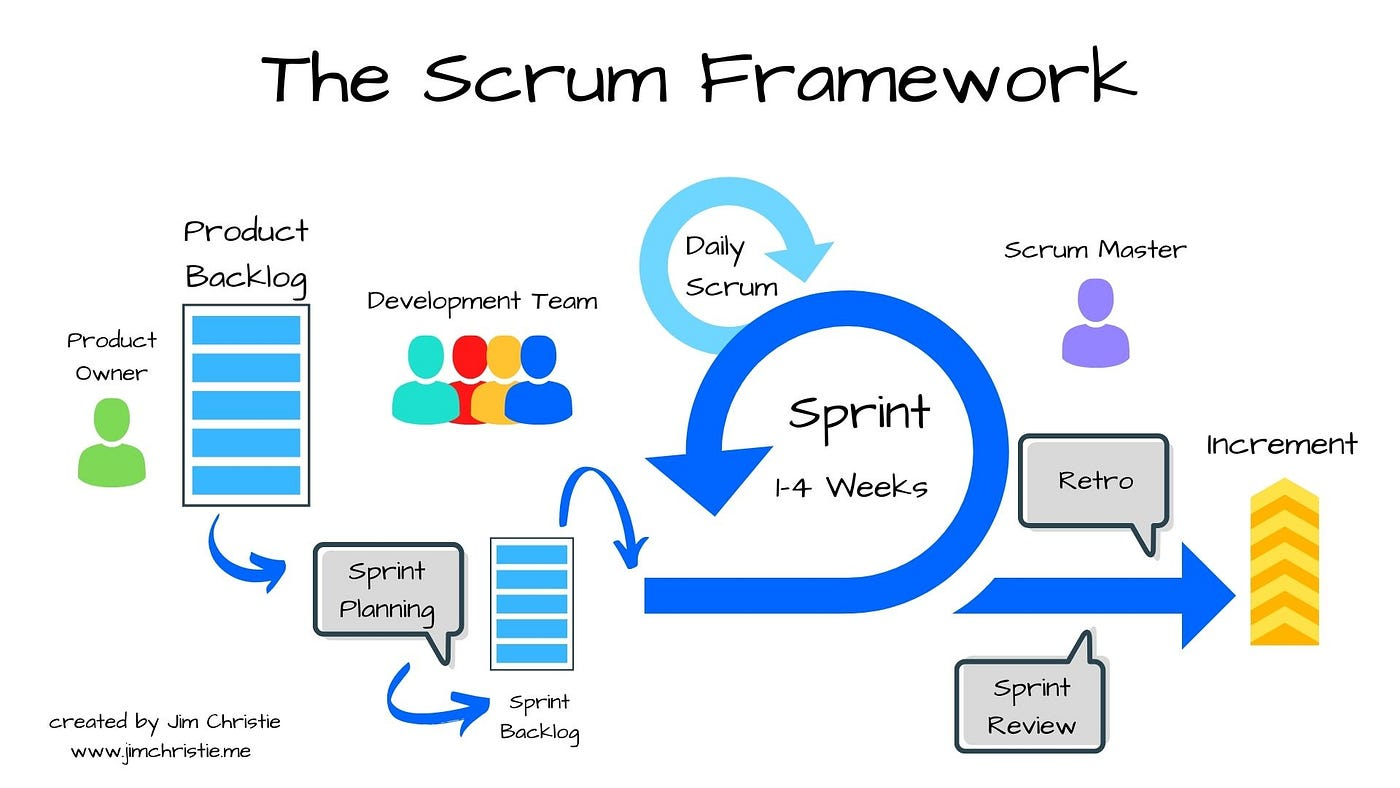
\includegraphics[alt={Schema del framework Scrum adottato}, width=0.9\linewidth]{img/framework_scrum.jpg}
    \caption{Schema semplificato del framework Scrum adottato}
    \label{fig:scrum-framework}
\end{figure}

\subsection{Comunicazione e documentazione}
La comunicazione avviene su canali Telegram dedicati a ciascun progetto, dove team e referenti si scambiano aggiornamenti quotidiani, e durante le cerimonie Scrum già descritte. Per la documentazione si utilizza la sezione \textit{Pages} di Plane, accessibile a tutti i membri del progetto, affiancata dai file nel repository (README, note operative). Per questo lavoro è presente anche una documentazione OpenAPI che descrive le REST API sviluppate.

\section{Strumenti tecnici e controllo qualità}

\subsection{Version control e branching}
Il codice è gestito con Git\footnote{\url{https://git-scm.com/}}, sistema di controllo versione distribuito, e ospitato su Gitea\footnote{\url{https://about.gitea.com/}}, piattaforma self-hosted per repository e merge request. È adottato un modello di branching ispirato a Gitflow ma ridotto alle necessità del progetto:
\begin{itemize}
    \item \textbf{main}: contiene le versioni rilasciabili e sincronizzate con l’ERP;
    \item \textbf{develop}: integra in modo continuo le attività in corso;
    \item \textbf{feature/<nome>}: per lo sviluppo di nuove funzionalità;
    \item \textbf{fix/<nome>}: per correggere errori individuati in test o review;
    \item \textbf{docs/<nome>}: per aggiornamenti alla documentazione.
\end{itemize}
Ogni branch è nominato in modo descrittivo per collegare rapidamente il lavoro all’attività tracciata.

I messaggi di commit seguono lo standard \textit{Conventional Commits}\footnote{\url{https://www.conventionalcommits.org/en/v1.0.0/}} con prefissi \texttt{feat}, \texttt{fix} e \texttt{docs}, così da facilitare la lettura della cronologia e la generazione di note di rilascio.

\begin{figure}[H]
    \centering
    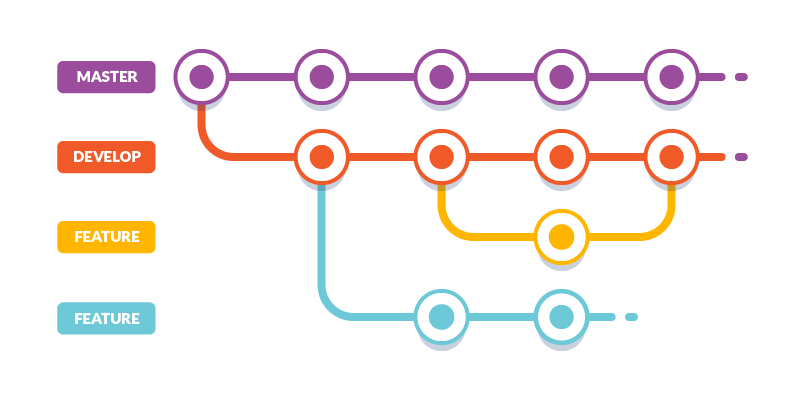
\includegraphics[alt={Schema del modello Gitflow adottato con branch main, develop e rami di feature/fix/docs}, width=0.9\linewidth]{img/gitflow_scheme.png}
    \caption{Schema del branching model adottato}
    \label{fig:gitflow-scheme}
\end{figure}

\subsection{Issue tracking}
Le attività sono tracciate su Plane\footnote{\url{https://plane.so}} con una board Kanban a quattro colonne: \textit{Backlog} raccoglie le attività proposte; \textit{Todo} contiene quelle selezionate per lo Sprint; \textit{In Progress} include il lavoro in corso; \textit{Done} raccoglie ciò che è completato.

Ogni issue include:
\begin{itemize}
\item descrizione chiara dell’attività, dell’obiettivo e dell’output atteso, sia esso una nuova feature, un bugfix o un aggiornamento documentale;
    \item livello di priorità, con valori \textit{Critical}, \textit{High}, \textit{Medium} o \textit{Low};
    \item assegnatario dell’attività, così da rendere esplicita la responsabilità e il punto di contatto;
    \item modulo del progetto a cui l’attività è collegata, utile per aggregare il lavoro per componente e verificare l’impatto.
\end{itemize}
\begin{figure}[H]
    \centering
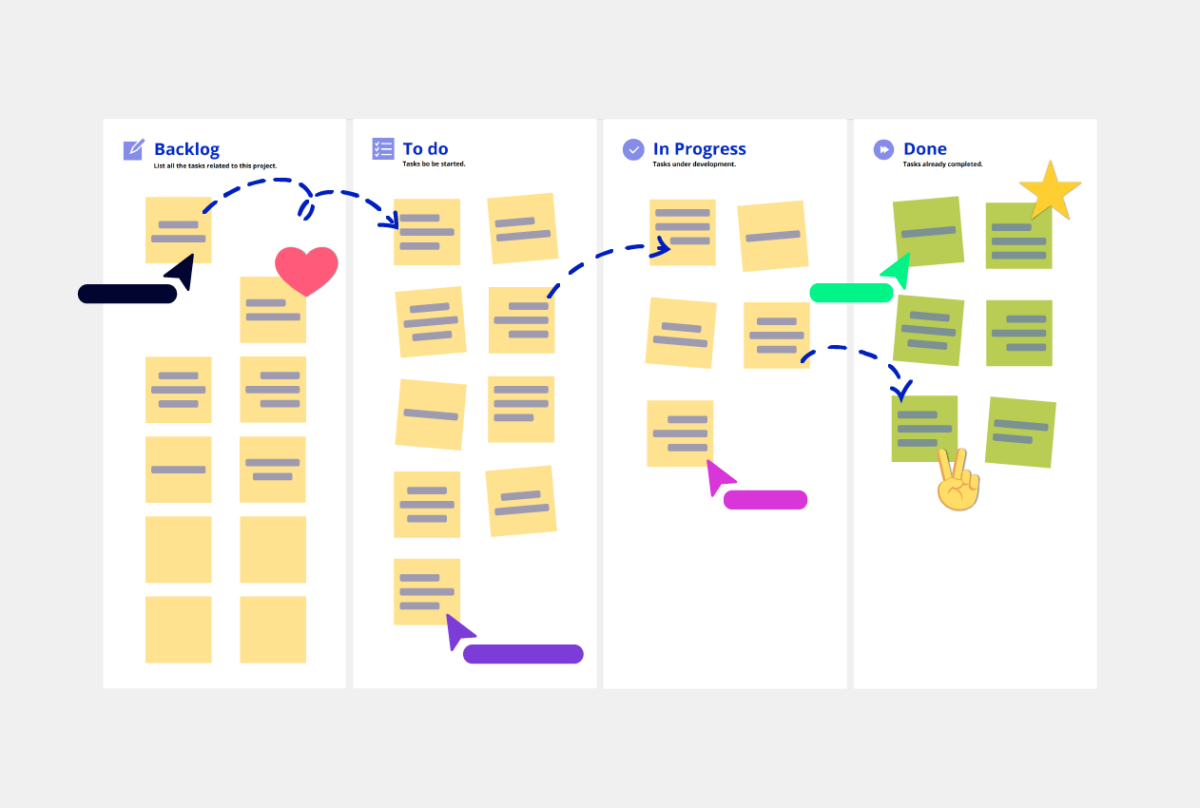
\includegraphics[alt={Esempio di board Kanban su Plane con colonne Backlog, Todo, In Progress, Done}, width=0.9\linewidth]{img/kanban_board.png}
    \caption{Schema semplificato della board Kanban su Plane}
    \label{fig:plane-board}
\end{figure}

\subsection{Testing e integrazione continua}
Per il modulo di previsione di \textit{ErpAI} è stata introdotta una pratica di integrazione continua approvata dall’azienda. Su Gitea è configurato un workflow che, a ogni push, esegue i test unitari sulle funzioni di pre-processing e sulle logiche di servizio, oltre ai test di integrazione sugli endpoint FastAPI. L’esito della pipeline è vincolante per questo modulo: solo i branch che superano i test possono essere mergiati in \texttt{main}, garantendo che il motore di previsione resti stabile prima di ogni distribuzione.



\newpage

    %\chapter{Descrizione dello stage}
\label{chap:descrizione-stage}

\section{Introduzione al progetto}
Il modulo di previsione sviluppato durante lo stage stima la domanda futura di prodotti finiti per supportare la pianificazione \gls{mrp} di \textit{ErpAI}. Le stime si basano sullo storico delle fatture di vendita e vengono propagate lungo le distinte base per evidenziare i fabbisogni di semilavorati e materie prime. I risultati vengono messi a disposizione dei planner come proposte rivedibili, affiancando inizialmente il processo manuale.

Obiettivi principali:
\begin{itemize}
    \item ridurre \textit{stock-out} e fermate impianto anticipando materiali critici;
    \item limitare \textit{overstock} e costi di magazzino evitando produzioni o acquisti non necessari;
    \item fornire previsioni integrabili con il modulo di \textit{planning} e l’interfaccia utente per approvare o modificare le proposte.
\end{itemize}


\section{Analisi preventiva dei rischi}

Durante la fase iniziale sono stati individuati alcuni rischi specifici per il modulo di previsione e la sua integrazione:

\begin{risk}{Qualità e quantità dei dati storici}
    \riskdescription{dati di vendita incompleti o disomogenei possono ridurre l’accuratezza del modello}
    \risksolution{pulizia e normalizzazione dei dataset, regole di validazione condivise con i referenti di business}
    \label{risk:data-quality}
\end{risk}

\begin{risk}{Integrazione con l’\gls{erp} e le \gls{api}}
    \riskdescription{ritardi o incongruenze nello scambio dati tra modulo di previsione, \textit{planning} e \gls{erp}}
    \risksolution{contratto \gls{api} documentato (OpenAPI), ambiente di staging per test end-to-end prima del rilascio}
    \label{risk:integration-api}
\end{risk}

\begin{risk}{Performance e tempi di risposta}
    \riskdescription{tempi di addestramento o interrogazione troppo lunghi per l’uso operativo}
    \risksolution{limitazione delle feature non essenziali, caching dei risultati, pianificazione di job batch fuori orario}
    \label{risk:performance}
\end{risk}

\begin{risk}{Qualità di generalizzazione del modello}
    \riskdescription{rischio di \gls{overfitting} o \gls{underfitting} a causa di dati sporchi o parametrizzazione non ottimale}
    \risksolution{pulizia e normalizzazione dei dati, regolarizzazione e ottimizzazione degli iperparametri per bilanciare complessità e capacità predittiva}
    \label{risk:model-generalization}
\end{risk}

\begin{risk}{Adozione da parte dei planner}
    \riskdescription{diffidenza verso i risultati del modello e ritardi nell’uso in produzione}
    \risksolution{esecuzione parallela al processo manuale per più cicli, raccolta \textit{feedback} e correzioni iterative}
    \label{risk:user-adoption}
\end{risk}

\section{Pianificazione}
\subsection{Modalità di stage e interazione}
Lo stage si svolge in presenza, con allineamenti quotidiani e tre \textit{touchpoint} settimanali con il tutor aziendale per supporto tecnico e validazione degli step. La comunicazione avviene di persona; il tutor fornisce revisione del codice, risoluzione problemi e verifica delle scelte progettuali.

\subsection{Pianificazione settimanale}
La Tabella~\ref{tab:pianificazione_settimanale} riporta la pianificazione delle attività settimanali concordata con il tutor aziendale all’inizio dello stage.
\begin{table}[htbp]
    \centering
    \renewcommand{\arraystretch}{1.2}
    \rowcolors{1}{}{tableGray}
    \begin{tabular}{|c|p{8cm}|c|}
    \hline
    \textbf{Settimana} & \textbf{Obiettivi/Attività} & \textbf{Ore}\\ \hline
    1 & Analisi requisiti e rischi; studio delle tecnologie da utilizzare. & 40\\ \hline
    2 & Progettazione e revisione della documentazione esistente. & 40\\ \hline
    3 & Codifica del progetto. & 40\\ \hline
    4 & Codifica del progetto. & 40\\ \hline
    5 & Codifica del progetto. & 40\\ \hline
    6 & Codifica del progetto. & 40\\ \hline
    7 & Codifica dei test e stesura della documentazione. & 40\\ \hline
    8 & Preparazione della presentazione finale, test conclusivi e chiusura attività. & 20\\ \hline
    \end{tabular}
    \caption{Pianificazione settimanale delle attività di stage.}
    \label{tab:pianificazione_settimanale}
\end{table}
\newpage

    %\chapter{Analisi dei requisiti}
\label{chap:analisi-requisiti}

\section{Casi d'uso}
In avvio di stage sono stati definiti requisiti e interazioni minime tra chi usa il gestionale e il motore di previsione, così da focalizzare solo i casi d’uso necessari alle previsioni.

\subsection{Attori individuati}
Gli attori che interagiscono con il motore di previsione sono:
\begin{itemize}
    \item \textbf{Utente finale}: usa l’interfaccia di ErpAI per avviare previsioni e consultare i risultati.
    \item \textbf{Gestionale ErpAI}: applicazione principale che inoltra le richieste al modulo di previsione via API protette, gestisce autenticazione e memorizza/mostra i risultati.
    \item \textbf{Modulo di previsione}: microservizio che aggiorna i dati, allena il modello, genera previsioni e notifica ErpAI via callback.
    \item \textbf{Modulo chatbot}: microservizio che può interrogare il modulo di previsione via API per ottenere previsioni e spiegazioni da usare nelle risposte.
\end{itemize}
L’interazione è orchestrata da ErpAI, che media verso il modulo di previsione e il chatbot.

\subsection{Casi d'uso}
\begin{center}
    \rowcolors{1}{}{tableGray}
    \begin{longtable}{|p{2.2cm}|p{11.8cm}|}
    \hline
    \multicolumn{1}{|c|}{\textbf{ID}} & \multicolumn{1}{c|}{\textbf{Descrizione}}\\
    \hline 
    \endfirsthead
    \rowcolor{white}
    \multicolumn{2}{c}{{\bfseries \tablename\ \thetable{} -- Continuo della tabella}}\\
    \hline
    \multicolumn{1}{|c|}{\textbf{ID}} & \multicolumn{1}{c|}{\textbf{Descrizione}}\\
    \hline 
    \endhead
    \hline
    \rowcolor{white}
    \multicolumn{2}{|r|}{{Continua nella prossima pagina...}}\\
    \hline
    \endfoot
    \endlastfoot 
    
    UC1 & \textbf{Attori}: Utente finale.\\
        & \textbf{Scopo}: Avviare una richiesta di previsione.\\
        & \textbf{Pre-condizione}: Autenticazione effettuata su ErpAI.\\
        & \textbf{Post-condizione}: Richiesta creata e inoltrata a ErpAI. \\ \hline
    UC1.1 & \textbf{Attori}: Utente finale.\\
        & \textbf{Scopo}: Selezionare l’intervallo temporale per la previsione.\\
        & \textbf{Pre-condizione}: Interfaccia di ErpAI aperta sulla schermata di previsione.\\
        & \textbf{Post-condizione}: Intervallo impostato. \\ \hline
    UC1.2 & \textbf{Attori}: Utente finale.\\
        & \textbf{Scopo}: Confermare e inviare la richiesta.\\
        & \textbf{Pre-condizione}: Parametri configurati (intervallo selezionato).\\
        & \textbf{Post-condizione}: Richiesta inviata a ErpAI. \\ \hline

    UC2 & \textbf{Attori}: Gestionale ErpAI.\\
        & \textbf{Scopo}: Inoltrare la richiesta al modulo di previsione.\\
        & \textbf{Pre-condizione}: Richiesta ricevuta dal frontend, API del modulo raggiungibile.\\
        & \textbf{Post-condizione}: Richiesta inoltrata. \\ \hline
    UC2.1 & \textbf{Attori}: Gestionale ErpAI.\\
        & \textbf{Scopo}: Richiedere token al modulo di previsione.\\
        & \textbf{Pre-condizione}: Credenziali client configurate.\\
        & \textbf{Post-condizione}: Token ricevuto oppure errore di autenticazione. \\ \hline
    UC2.2 & \textbf{Attori}: Gestionale ErpAI.\\
        & \textbf{Scopo}: Inviare la richiesta con token al modulo di previsione.\\
        & \textbf{Pre-condizione}: Token valido, parametri di previsione disponibili.\\
        & \textbf{Post-condizione}: Richiesta accettata o errore ricevuto. \\ \hline

    UC3 & \textbf{Attori}: Modulo di previsione.\\
        & \textbf{Scopo}: Processare la previsione e notificare ErpAI.\\
        & \textbf{Pre-condizione}: Richiesta UC2.2 ricevuta e valida.\\
        & \textbf{Post-condizione}: Previsione elaborata o errore rilevato. \\ \hline
    UC3.1 & \textbf{Attori}: Modulo di previsione.\\
        & \textbf{Scopo}: Elaborare dati e generare previsione.\\
        & \textbf{Pre-condizione}: Richiesta valida.\\
        & \textbf{Post-condizione}: Previsione pronta oppure errore registrato. \\ \hline
    UC3.2 & \textbf{Attori}: Modulo di previsione.\\
        & \textbf{Scopo}: Notificare il completamento a ErpAI.\\
        & \textbf{Pre-condizione}: Processo terminato (successo o fallimento).\\
        & \textbf{Post-condizione}: Stato aggiornato in ErpAI. \\ \hline
    UC3.E & \textbf{Attori}: Modulo di previsione.\\
        & \textbf{Scopo}: Notificare errore a ErpAI.\\
        & \textbf{Pre-condizione}: Errore registrato durante UC3.1.\\
        & \textbf{Post-condizione}: Stato marcato come fallito in ErpAI. \\ \hline

    UC4 & \textbf{Attori}: Modulo Chatbot.\\
        & \textbf{Scopo}: Richiedere contesto previsione.\\
        & \textbf{Pre-condizione}: Chatbot autorizzato verso le API del modulo di previsione.\\
        & \textbf{Post-condizione}: Richieste pronte o dati ricevuti/errore gestito. \\ \hline
    UC4.1 & \textbf{Attori}: Modulo Chatbot.\\
        & \textbf{Scopo}: Preparare richiesta e token.\\
        & \textbf{Pre-condizione}: Credenziali client configurate.\\
        & \textbf{Post-condizione}: Token ricevuto oppure errore di autenticazione. \\ \hline
    UC4.2 & \textbf{Attori}: Modulo Chatbot.\\
        & \textbf{Scopo}: Recuperare dati previsionali via API.\\
        & \textbf{Pre-condizione}: Token valido, ID previsione noto.\\
        & \textbf{Post-condizione}: Dati ricevuti oppure errore gestito. \\ \hline
    UC4.E & \textbf{Attori}: Modulo Chatbot.\\
        & \textbf{Scopo}: Gestire errore API.\\
        & \textbf{Pre-condizione}: Errore nelle chiamate di UC4.1 o UC4.2.\\
        & \textbf{Post-condizione}: Errore registrato, risposta di errore al chiamante. \\ \hline
    \end{longtable}
\end{center}

\begin{figure}[H]
    \centering
    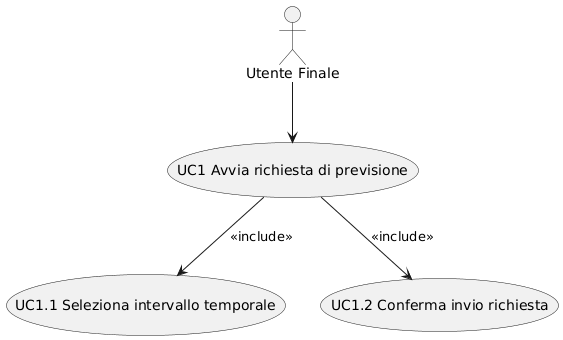
\includegraphics[width=\linewidth]{img/usecase/usecase1.png}
    \caption{Use case 1: avvio e invio richiesta di previsione}
\end{figure}

\begin{figure}[H]
    \centering
    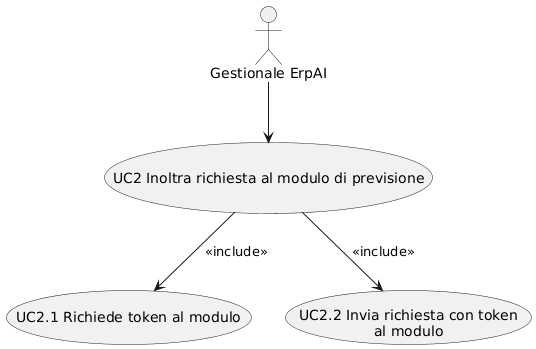
\includegraphics[width=\linewidth]{img/usecase/usecase2.png}
    \caption{Use case 2: inoltro della richiesta da ErpAI al modulo di previsione}
\end{figure}

\begin{figure}[H]
    \centering
    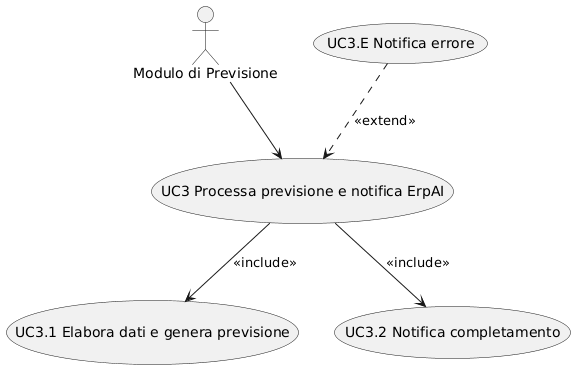
\includegraphics[width=\linewidth]{img/usecase/usecase3.png}
    \caption{Use case 3: elaborazione e notifica da parte del modulo di previsione}
\end{figure}

\begin{figure}[H]
    \centering
    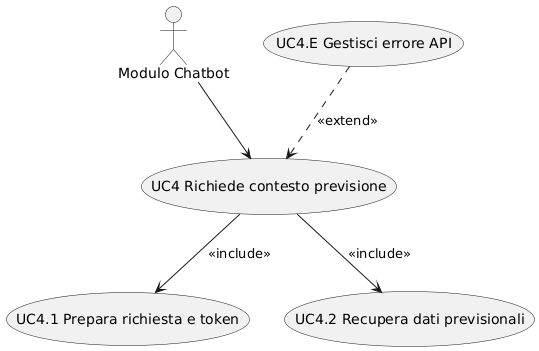
\includegraphics[width=\linewidth]{img/usecase/usecase4.png}
    \caption{Use case 4: interazione del modulo chatbot con il modulo di previsione}
\end{figure}

\section{Requisiti}
Questa sezione raccoglie i requisiti del progetto di previsione e pianificazione per \textit{ErpAI}, organizzati in obbligatori (O), desiderabili (D) e facoltativi (F). La codifica usa un prefisso che identifica la priorità (O/D/F) seguito da un numero progressivo.

\begin{center}
    \rowcolors{1}{}{tableGray}
    \begin{longtable}{|p{2cm}|p{9cm}|p{3cm}|}
    \hline
    \multicolumn{1}{|c|}{\textbf{ID}} & \multicolumn{1}{c|}{\textbf{Descrizione}} & \multicolumn{1}{c|}{\textbf{Categoria}}\\
    \hline 
    \endfirsthead
    \rowcolor{white}
    \multicolumn{3}{c}{{\bfseries \tablename\ \thetable{} -- Continuo della tabella}}\\
    \hline
    \multicolumn{1}{|c|}{\textbf{ID}} & \multicolumn{1}{c|}{\textbf{Descrizione}} & \multicolumn{1}{c|}{\textbf{Categoria}}\\
    \hline 
    \endhead
    \hline
    \rowcolor{white}
    \multicolumn{3}{|r|}{{Continua nella prossima pagina...}}\\
    \hline
    \endfoot
    \endlastfoot 
    
    O01 & Data-set e data-model consolidati. & Obbligatorio \\ \hline
    O02 & Pipeline di previsione con intervalli di confidenza. & Obbligatorio \\ \hline
    O03 & Motore MRP con piani compatibili con lead-time e scorte minime. & Obbligatorio \\ \hline
    D01 & Logica base di feedback learning da input dell’operatore. & Desiderabile \\ \hline
    D02 & Automazione della valutazione delle spiegazioni. & Desiderabile \\ \hline
    D03 & Simulazione dell’impatto delle azioni correttive nel tempo. & Desiderabile \\ \hline
    F01 & Prototipazione grafica per output prescrittivi. & Facoltativo \\ \hline
    F02 & Estensione a scenari multi-macchina. & Facoltativo \\ \hline
    F03 & Integrazione con notifiche real-time per allarmi e azioni. & Facoltativo \\ \hline
    \end{longtable}
\end{center}

\newpage

    %\chapter{Progettazione}
\label{chap:design}
Una parte consistente del monte ore iniziale dello stage è stata investita nella fase di progettazione: definizione dell’architettura del modulo di previsione, individuazione dei confini funzionali e selezione degli strumenti. Le prime settimane sono state dedicate alla prova comparativa delle tecnologie (modello, \gls{api}, orchestrazione), allo studio della documentazione ufficiale e alla costruzione di prototipi rapidi; ciò ha permesso di arrivare alla fase successiva con scelte già validate e di avviare lo sviluppo su basi stabili.

\section{Tecnologie e strumenti}
\label{sec:tecnologie-strumenti}
In questa sezione sono elencate le principali tecnologie e librerie adottate per lo sviluppo del modulo di previsione, con una breve descrizione delle loro funzionalità.

\subsection{Linguaggi di programmazione}
\begin{itemize}
    \item \textbf{Python}\footnote{\url{https://www.python.org/}}: linguaggio di programmazione interpretato, ad alto livello e tipizzato dinamicamente, progettato per leggibilità e rapidità di sviluppo. Offre un vasto ecosistema di librerie per calcolo scientifico, machine learning e sviluppo applicativo.
    \item \textbf{SQL}: è un linguaggio dichiarativo standardizzato per definire, interrogare e manipolare dati all’interno di database relazionali. Fornisce strumenti per creare schemi, gestire transazioni ed eseguire query complesse in modo ottimizzato. È il mezzo principale per accedere e gestire dati strutturati in sistemi informativi.
    
\end{itemize}

\subsection{Framework e server web}
\begin{itemize}
    \item \textbf{FastAPI}\footnote{\url{https://fastapi.tiangolo.com/}}: FastAPI è un \textit{framework} web Python ad alte prestazioni per la creazione di \gls{api} basate su standard come OpenAPI e JSON Schema. Utilizza tipizzazione Python e Pydantic per validazione automatica e autogenerazione della documentazione.
    \item \textbf{Uvicorn}: server \gls{asgi} leggero e ad alte prestazioni, basato su uvloop e httptools, progettato per applicazioni web asincrone in Python. Fornisce un runtime veloce e a bassa latenza ideale per \textit{framework} come FastAPI.
\end{itemize}

\subsection{Database e ORM}
\begin{itemize}
    \item \textbf{SQLAlchemy}: toolkit SQL e ORM per Python che fornisce un livello di astrazione avanzato per interagire con database relazionali.
    \item \textbf{Alembic}\footnote{\url{https://alembic.sqlalchemy.org/}}: strumento di database migration per SQLAlchemy che gestisce in modo versionato l’evoluzione degli schemi relazionali. Permette di generare, applicare e monitorare migrazioni tramite script incrementali.
    \item \textbf{DuckDB}: è un database analitico in-process orientato alle query OLAP, progettato per esecuzioni ad alte prestazioni direttamente all’interno dell’applicazione. Utilizza un motore vettorizzato e columnar per elaborare rapidamente grandi dataset senza necessità di un server esterno.
    \item \textbf{ChromaDB}: database vettoriale progettato per l’indicizzazione e la ricerca semantica tramite \gls{embedding} ad alta dimensionalità. Fornisce storage ottimizzato, funzioni di \gls{similaritysearch} e gestione di metadata per applicazioni \gls{llm} e retrieval-augmented.
\end{itemize}

\subsection{Autenticazione e sicurezza}
\begin{itemize}
    \item \textbf{PyJWT}\footnote{\url{https://pyjwt.readthedocs.io/}}: libreria Python per creare, firmare e validare \gls{jwt}, utilizzati per autenticazione e scambio sicuro di informazioni.
\end{itemize}

\subsection{Machine Learning e Data Science}
\begin{itemize}
    \item \textbf{Pydantic}\footnote{\url{https://pydantic.dev/}}: libreria Python per la validazione e la gestione di dati basata su annotazioni di tipo. Consente di definire modelli di dati con tipi forti, validazione automatica e serializzazione/deserializzazione in modo semplice ed efficiente.
    \item \textbf{Pandas}: libreria Python per la manipolazione e l’analisi di dati strutturati, basata su oggetti fondamentali come DataFrame e Series. Offre strumenti ad alte prestazioni per filtrare, trasformare, aggregare e pulire dataset.
    \item \textbf{NumPy}: libreria Python per il calcolo scientifico che fornisce array n-dimensionali ad alte prestazioni e operazioni vettorializzate. Include funzioni per algebra lineare, statistica e trasformazioni numeriche ottimizzate in C.
    \item \textbf{scikit-learn}: libreria Python per il machine learning che offre algoritmi efficienti per classificazione, regressione, clustering e riduzione della dimensionalità. Fornisce \acrshort{api} uniformi, strumenti per preprocessing, valutazione dei modelli e pipeline.
    \item \textbf{XGBoost}\footnote{\url{https://xgboost.ai/}}: libreria Python ottimizzata per gradient boosting che implementa alberi decisionali ad alte prestazioni, pensata per competizioni di machine learning e applicazioni industriali. Utilizza parallelismo, pruning avanzato e ottimizzazioni su memoria e \acrshort{gpu}. È nota per l’elevata accuratezza e l’efficienza su grandi dataset tabulari.
    \item \textbf{\acrshort{shap}}\footnote{\url{https://shap.readthedocs.io/}}: libreria Python che fornisce metodi basati sui valori di Shapley per interpretare modelli di machine learning. Calcola contributi locali e globali delle feature alle predizioni. È ampiamente utilizzata per garantire trasparenza, explainability e analisi di modelli complessi come XGBoost
\end{itemize}

\subsection{Strumenti di testing e deployment}
\begin{itemize}
    \item \textbf{Pytest}: \textit{framework} di testing per Python che permette di scrivere test semplici, modulari e scalabili tramite un approccio basato su funzioni e fixture. Supporta parametric testing, plugin estendibili e rilevamento automatico dei test.
    \item \textbf{Docker}\footnote{\url{https://www.docker.com/}}: piattaforma di containerizzazione che consente di impacchettare applicazioni e dipendenze in ambienti isolati e portabili chiamati container. Utilizza un motore leggero basato su immagini stratificate per garantire coerenza tra ambienti di sviluppo, test e produzione. Facilita il deployment scalabile e riproducibile di applicazioni moderne.
\end{itemize}

\section{Architettura}
\label{sec:architettura}

L’architettura complessiva del sistema \ref{fig:architettura-generale} è stata progettata secondo principi di modularità e componibilità, in modo da permettere l’evoluzione indipendente dei singoli blocchi funzionali. 
Il modulo \textit{ErpAI-Forecasting} si inserisce come componente aggiuntivo della piattaforma \textit{ErpAI} e fornisce funzionalità di previsione basate su modelli di machine learning. 
Tutte le comunicazioni verso il modulo avvengono tramite l’\gls{api} Gateway, che gestisce la validazione dei token \acrshort{jwt} presso l’Auth Server, l’instradamento delle richieste e l’esposizione controllata delle \acrshort{api} pubbliche e interne. 

L’orchestrazione vera e propria è realizzata all’interno del Modulo di Previsione, che combina tre elementi chiave: dati \gls{erp} sincronizzati tramite DuckDB, un modello XGBoost ottimizzato per il dominio applicativo, e un sistema di persistenza distribuito che comprende Prevision DB e Chroma DB. 
Questa architettura permette di separare nettamente l’elaborazione analitica (DuckDB), l’inferenza e l’explainability (Modulo di Previsione) e la persistenza (Prevision DB / Chroma DB).  
La presenza di contratti ben definiti (schema delle \acrshort{api} \acrshort{rest}, modelli Pydantic, formati dei dataset e versioning dei modelli) garantisce la possibilità di sostituire o aggiornare ciascun componente senza introdurre impatti a catena sugli altri servizi.

\begin{figure}[H]
    \centering
    \makebox[\textwidth][c]{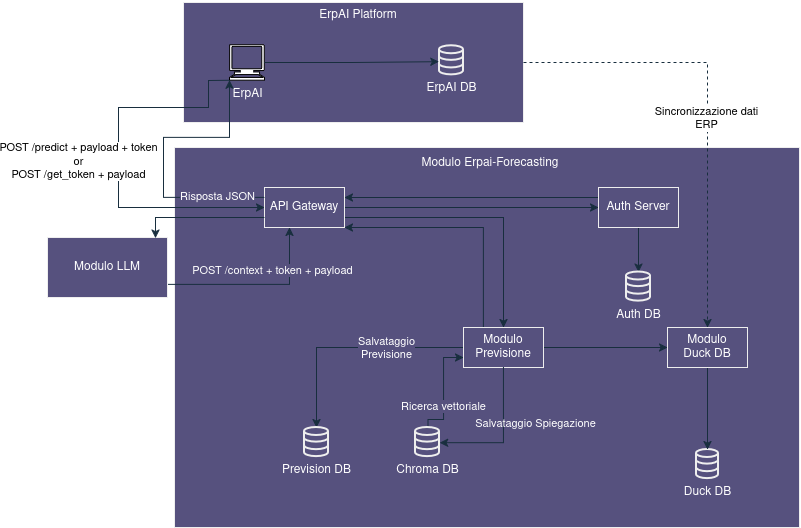
\includegraphics[width=1.1\linewidth]{img/Architettura_1.png}}
    \caption{Architettura complessiva del modulo ErpAI-Forecasting}
    \label{fig:architettura-generale}
\end{figure}

\subsection{API Gateway}
Il sistema utilizza Kong\footnote{\url{https://konghq.com/}} come \gls{api} Gateway per garantire un unico punto di ingresso alle \gls{api} esposte dal modulo \textit{ErpAI-Forecasting}.  
Kong gestisce instradamento, rate limiting, logging e policy di sicurezza, consentendo di centralizzare funzioni trasversali che altrimenti dovrebbero essere replicate nei singoli servizi.  
Ogni richiesta proveniente da \textit{ErpAI} o dal Modulo \acrshort{llm} viene validata e inoltrata al Modulo di Previsione solo dopo la verifica del token \acrshort{jwt}.

\subsection{Auth Server}
L’Auth Server è responsabile dell’autenticazione e dell’emissione dei token \acrshort{jwt}.  
Espone endpoint per la richiesta di credenziali, la validazione dei token e la gestione di client applicativi autorizzati.  
Si appoggia ad Auth DB per memorizzare utenti, ruoli e chiavi pubbliche/privati necessarie alla firma e alla verifica dei token.  
L’\acrshort{api} Gateway consulta l’Auth Server (o i suoi metadati \acrshort{jwks}) per validare l’autenticità delle richieste in ingresso.

\subsection{Modulo DuckDB}
DuckDB è il database embedded, analitico e in-process orientato a query \gls{olap} che alimenta il forecasting e ospita la replica dei dati \acrshort{erp}. La configurazione legge l’URL da \texttt{DUCKDB\_URL} (o \texttt{DUCKDB\_DATABASE\_URL} nel servizio di sync), costruisce il percorso su filesystem e, se la directory non è scrivibile, ripiega su un file locale in sola lettura quando già esistente. Il \textit{repository} di forecasting espone \texttt{fetch\_fact\_invoices}, che restituisce \texttt{fact\_invoices} come DataFrame Pandas da usare per normalizzazione e preparazione dei dataset.
\begin{itemize}
    \item \textbf{Sincronizzazione}: un servizio di orchestrazione preleva i dati \acrshort{erp} attraverso i seguenti metodi:
    \begin{itemize}
        \item \textbf{fetch\_invoices}: sincronizza la tabella \texttt{invoices} con le informazioni delle fatture di vendita emesse.
        \item \textbf{fetch\_articles}: sincronizza la tabella \texttt{articles} con tutti gli articoli in vendita.
        \item \textbf{fetch\_customers}: sincronizza la tabella \texttt{customers} con l’anagrafica clienti.
        \item \textbf{fetch\_vat\_options}: sincronizza la tabella \texttt{vat\_options} con le aliquote IVA.
        \item \textbf{fetch\_article\_invoice}: sincronizza la tabella \texttt{article\_invoice} con le righe degli articoli presenti nelle fatture.
    \end{itemize}
    \item \textbf{Costruzione di \texttt{fact\_invoices}}: dopo la sincronizzazione viene ricreata la tabella \texttt{fact\_invoices}, che aggrega le informazioni rilevanti per il forecasting calcolando metriche come il totale fatturato per cliente, articolo e periodo.
\end{itemize}

\subsection{Modulo di Previsione}
Il Modulo di Previsione orchestrato da FastAPI gestisce l’intero ciclo di inferenza, dall’accesso ai dati fino alla persistenza dei risultati. Gli endpoint \acrshort{rest} validano il payload (Pydantic), avviano un job tracciato e coordinano i servizi sottostanti:
\begin{itemize}
    \item \textbf{Acquisizione dati}: lettura delle \texttt{fact\_invoices} da DuckDB, normalizzazione di colonne/tempi e copertura mensile per articolo; filtri opzionali sulla data di cutoff.
    \item \textbf{\gls{featureengineering}}: costruzione del dataframe utilizzato per il training del modello e aggiunta di feature derivate come lag, rolling, trend stagionali e indicatori temporali.
    \item \textbf{Inferenza XGBoost}: allenamento del modello XGBoost sui dati raccolti e generazione delle previsioni per il periodo richiesto con calcolo delle metriche di accuratezza come \gls{mape}, \gls{wape} e \gls{rmse}.
    \item \textbf{Spiegazioni \acrshort{shap}}: calcolo dei valori \acrshort{shap} per ogni previsione generata, con estrazione delle feature più influenti.
    \item \textbf{Persistenza}: i risulrttati numerici, le spiegazioni e le metriche vengono salvati in Prevision DB e Chroma DB per consentire consultazioni future e audit dei processi.
    \item \textbf{Notifiche e callback}: al termine del job di previsione viene inviata una notifica di completamento ad \textit{ErpAI} tramite \gls{callback} \gls{http}, includendo lo stato e i riferimenti ai risultati salvati.
\end{itemize}

\subsection{Prevision DB}
Prevision DB conserva job, run di previsione e righe di output. Le principali tabelle sono:
\begin{itemize}
    \item \textbf{jobs}: contiene i job di previsione ed è composta da:
    \begin{itemize}
        \item \textbf{id}: identificativo univoco del job.
        \item \textbf{status}: stato del job (in coda, in esecuzione, completato, fallito).
        \item \textbf{detail}: dettaglio/errore se presente.
        \item \textbf{dataset\_id}: riferimento al dataset sincronizzato usato dal job.
        \item \textbf{timestamp}: creazione, avvio, fine ed ultimo aggiornamento.
    \end{itemize}
    \item \textbf{forecast\_runs}: registra le esecuzioni di previsione, con:
    \begin{itemize}
        \item \textbf{id}: identificativo del run.
        \item \textbf{mape}: metrica di errore della previsione usata per valutare la run.
        \item \textbf{created\_at}: data e ora di creazione della run.
    \end{itemize}
    \item \textbf{predictions\_xgboost}: contiene le righe previsionali, con:
    \begin{itemize}
        \item \textbf{forecast\_id}: riferimento alla run che ha generato la previsione.
        \item \textbf{article\_id} e \textbf{article\_name}: articolo a cui si riferisce la previsione.
        \item \textbf{prediction\_date}: data della previsione.
        \item \textbf{predicted\_quantity}: quantità stimata.
    \end{itemize}
\end{itemize}
La struttura dei dati consente di collegare job, run e singole previsioni, supportando consultazioni e analisi successive.

\subsection{Chroma DB}
Chroma DB è l’archivio vettoriale che memorizza \gls{embedding}, previsioni e spiegazioni, organizzate in due collection collegate da un ID di run nei metadati:
\begin{itemize}
    \item \textbf{prevision\_collection}: contiene le previsioni (article\_id, article\_name, data, quantità prevista) con \gls{embedding} e metadati della run.
    \item \textbf{explanation\_collection}: memorizza le spiegazioni \acrshort{shap} per ogni previsione, con metadati che riferiscono alla stessa run e all’articolo.
\end{itemize}
Le due collection permettono ricerche semantiche su risultati e spiegazioni e il collegamento rapido alla run e all’articolo, a supporto del Modulo \acrshort{llm} tramite \gls{embedding}.

\subsection{Auth DB}
Auth DB gestisce le credenziali dei client applicativi tramite la tabella \texttt{clients}, composta da:
\begin{itemize}
    \item \textbf{id}: identificativo della riga.
    \item \textbf{client\_id}: identificativo pubblico del client.
    \item \textbf{client\_secret}: segreto usato per autenticare il client.
    \item \textbf{is\_active}: flag che abilita o disabilita il client.
\end{itemize}
L’Auth Server consulta questa tabella per verificare e autorizzare i client in ingresso.

\section{Design pattern adottati}
\label{sec:design-pattern}
In questa sezione sono riassunti i pattern architetturali e di inversione del controllo adottati, con l’obiettivo di separare le responsabilità, semplificare lo sviluppo e rendere il modulo facilmente testabile e manutenibile.

\subsection{Architettura a layer}
L’architettura del modulo di previsione è organizzata a layer, ogni layer ha responsabilità ben definite e comunica solo con i layer adiacenti in un approccio \emph{closed layer}.
Il vantaggio principale di questa struttura è la separazione delle responsabilità, che consente di isolare la logica di business dalla gestione delle \acrshort{api} e dall’accesso ai dati.
\textbf{Layer implementati}:
\begin{itemize}
    \item \textbf{API Layer}: espone \acrshort{api} \acrshort{rest} (FastAPI), valida i payload e avvia il flusso; nessuna logica di dominio né accesso diretto ai dati.
    \item \textbf{Business Layer}: logica business del modulo di previsione, riceve \gls{dto} dalle \gls{api} e effettua le operazioni necessarie orchestrando i servizi sottostanti.
    \item \textbf{Persistence Layer}: collega il business layer ai database esterni tramite \textit{repository} dedicati; incapsula logica di accesso ai dati e query SQL.
    \item \textbf{Database Layer}: contiene i database del sistema. dove i dati sono effettivamente memorizzati.
\end{itemize}

\subsection{Repository pattern}
Il sistema adotta il \gls{repositorypattern} per isolare completamente la logica di accesso ai dati dai servizi applicativi. Ogni database o storage esterno (relazionale, vettoriale o analitico) è incapsulato in un \textit{repository} dedicato che espone metodi di alto livello per \acrshort{crud} e query di dominio. Questa astrazione mantiene i servizi indipendenti dall’implementazione fisica del dato, semplifica l’integrazione con backend diversi, migliora la testabilità tramite mock e accelera la sostituzione o l’evoluzione dei motori di persistenza.
Lo snippet \ref{listing:repository-pattern} mostra un esempio di \textit{repository} per Chroma DB.
\begin{itemize}
    \item \textbf{ForecastRepository}: accesso a Prevision DB (creazione job, salvataggio run, metriche, righe previsionali).
    \item \textbf{DuckDBRepository}: accesso a DuckDB (\texttt{fact\_invoices} come DataFrame Pandas).
    \item \textbf{ChromaRepository}: accesso a Chroma DB (salvataggio/interrogazione embedding e metadati semantici).
\end{itemize}

\captionsetup{type=listing, belowskip=0pt}
\inputminted[fontsize=\small, breaklines, breakanywhere=true, linenos=true, bgcolor=gray!10]{python}{code/repository_pattern.py}
\captionof{listing}{Esempio di \textit{repository} per Chroma.}
\label{listing:repository-pattern}

\subsection{Inversione del controllo}
Il modulo di previsione utilizza il principio di Inversion of Control tramite Dependency Injection per gestire le relazioni tra i vari componenti del sistema.
In pratica, i servizi non creano direttamente gli oggetti di cui hanno bisogno, ma li ricevono già pronti dall’esterno, ad esempio tramite il costruttore.
Questo approccio rende il codice più ordinato e facile da mantenere, perché ogni componente è meno dipendente dagli altri.
Permette inoltre di sostituire rapidamente una parte del sistema senza modificare il resto dell’applicazione, e semplifica molto anche la fase di test, dove è possibile fornire versioni simulate delle dipendenze.
Lo snippet \ref{listing:dependency-injection} mostra un esempio di dependency injection in \texttt{ForecastService}.
\captionsetup{type=listing, belowskip=0pt}
\inputminted[fontsize=\small, breaklines, breakanywhere=true, linenos=true, bgcolor=gray!10]{python}{code/dependency_injection.py}
\captionof{listing}{Esempio di dependency injection.}
\label{listing:dependency-injection}

    %\chapter{Codifica}
\label{chap:code}
Gran parte del periodo di stage è stata dedicata allo sviluppo del codice che realizza il sistema di previsione descritto nei capitoli precedenti.
In questo capitolo vengono presentate l’organizzazione della codebase e le principali logiche applicative che la compongono.

\section{Struttura del codice}
\label{chap:codebase}
La struttura delle directory del progetto è organizzata per separare chiaramente i vari componenti e facilitare la navigazione del codice (Figura~\ref{fig:repo-structure}).
Di seguito è riportata una descrizione delle principali cartelle e file presenti nel repository.
\subsection{Root}
\begin{itemize}
    \item \textbf{ErpAI-Forecasting/}: cartella principale del progetto contenente tutto il codice sorgente.
    \begin{itemize}
        \item \textbf{.gitea/}: cartella contenente le configurazioni per l’integrazione continua con Gitea.
        \item \textbf{auth-server/}: modulo di autenticazione.
        \item \textbf{forecasting/}: modulo principale del sistema.
        \item \textbf{duckdb/}: servizio di sincronizzazione dati ERP con scheduler mensile.
        \item \textbf{kong/}: cartella contenente la configurazione del gateway API che espone i servizi interni.
        \item \textbf{openapi/}: servizio che pubblica la documentazione ERP.
        \item \textbf{.env}: variabili d’ambiente.
        \item \textbf{.gitignore}: file di esclusione git.
        \item \textbf{alembic.ini}: configurazione di Alembic per le migrazioni del database.
        \item \textbf{compose.base.yml}: definizione Docker Compose base.
        \item \textbf{compose.yml}: definizione Docker Compose principale.
        \item \textbf{Dockerfile}: build dell’immagine principale.
        \item \textbf{pytest.ini}: configurazioni per i test.
        \item \textbf{README.md}: documentazione di progetto.
    \end{itemize}
\end{itemize}
\subsection{forecasting}
Approfondiamo il modulo di previsione in quanto cuore del sistema e oggetto principale di questo lavoro di tesi.
\begin{itemize}
    \item \textbf{app/}: cartella principale del modulo di previsione.
    \begin{itemize}
        \item \textbf{api/}: cartella che contiene i router FastAPI per gli endpoint REST.
        \item \textbf{db/}: cartella che contiene engine e setup DB locale.
        \item \textbf{dependencies/}: cartella che contiene la configurazione per la dependency injection.
        \item \textbf{models/}: cartella che contiene i modelli Pydantic e SQLModel per payload e tabelle.
        \item \textbf{repositories/}: cartella che contiene le implementazioni del repository pattern per l’accesso ai database esterni.
        \item \textbf{services/}: cartella che contiene le classi che implementano la logica di business e orchestrazione del flusso di previsione.
    \end{itemize}
    \item \textbf{chroma-data/}: cartella che contiene i dati persistenti di Chroma DB.
    \item \textbf{graphs/}: cartella che contiene gli output grafici SHAP generati.
    \item \textbf{migrations/}: cartella che contiene gli script Alembic per la gestione delle migrazioni del database.
    \item \textbf{tests/}: cartella che contiene la suite di test.
    \item \textbf{compose.forecasting.yml}: definizione Docker Compose specifica per il servizio forecasting.
    \item \textbf{Dockerfile}: build dell’immagine del servizio forecasting.
    \item \textbf{requirements.txt}: dipendenze Python.
\end{itemize}

\begin{figure}[H]
    \centering
    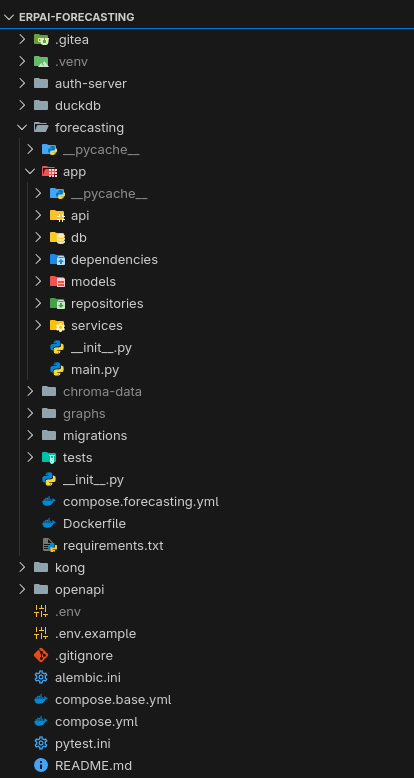
\includegraphics[width=0.6\linewidth]{img/repository.png}
    \caption{Struttura delle directory del progetto.}
    \label{fig:repo-structure}
\end{figure}

\section{Modelli dei dati}
\label{sec:code-models}
Nella cartella \texttt{models/} si trovano i modelli utilizzati per descrivere in modo tipizzato i dati che attraversano l’applicazione: gli schema Pydantic definiscono i payload di richiesta e risposta esposti dalle API FastAPI, mentre i modelli SQLModel rappresentano le tabelle e le relazioni persistite nei database operazionali. Di seguito sono riportati i principali modelli implementati, con una breve descrizione dei campi e il codice di riferimento.
\subsection{Modelli Pydantic}
\subsubsection{Article}
Questo modello definisce e valida un articolo del catalogo prodotti. Ogni \texttt{Article} è composto dai seguenti campi:
\begin{itemize}
    \item \textbf{id}: intero che identifica univocamente l’articolo.
    \item \textbf{name}: stringa con il nome dell’articolo.
    \item \textbf{code}: stringa con il codice identificativo.
    \item \textbf{vat}: numero (float) con l’aliquota IVA associata.
\end{itemize}

\begin{listing}[H]
\inputminted[fontsize=\small, breaklines, breakanywhere=true, linenos=true, bgcolor=gray!10]{python}{code/models/article.py}
\caption{Modello Pydantic \texttt{Article} (\texttt{models/article.py}).}
\label{listing:model-article}
\end{listing}

\subsubsection{Invoice}
Questo modello definisce e valida una fattura con le sue righe di dettaglio. Ogni \texttt{Invoice} include:
\begin{itemize}
    \item \textbf{id}: intero identificativo della fattura.
    \item \textbf{customer}: stringa con l’anagrafica cliente.
    \item \textbf{creating\_date}: data di emissione.
    \item \textbf{expiring\_date}: data di scadenza (opzionale).
    \item \textbf{expected\_shipping\_date} / \textbf{real\_shipping\_date}: date di spedizione prevista/effectiva (opzionali).
    \item \textbf{total}: numero (float) dell’importo totale.
    \item \textbf{articles}: lista di righe articolo (\texttt{ArticleInvoice}).
\end{itemize}
\begin{listing}[H]
\inputminted[fontsize=\small, breaklines, breakanywhere=true, linenos=true, bgcolor=gray!10]{python}{code/models/invoice.py}
\caption{Modello Pydantic \texttt{Invoice} (\texttt{models/invoice.py}).}
\label{listing:model-invoice}
\end{listing}

\subsubsection{Job, JobKind, JobStatus}
Questi modelli definiscono e validano i job di training/forecasting e il loro ciclo di vita. I campi principali sono:
\begin{itemize}
    \item \textbf{job\_id}: stringa identificativa del job.
    \item \textbf{status}: enum con stato corrente (\texttt{queued}, \texttt{running}, \texttt{succeeded}, \texttt{failed}).
    \item \textbf{kind}: enum con il tipo di job (\texttt{training} o \texttt{forecasting}).
    \item \textbf{detail}: stringa opzionale con dettagli/errore.
    \item \textbf{created\_at}, \textbf{started\_at}, \textbf{finished\_at}: timestamp (stringa) di creazione, avvio e fine (opzionali).
\end{itemize}
\begin{listing}[H]
\inputminted[fontsize=\small, breaklines, breakanywhere=true, linenos=true, bgcolor=gray!10]{python}{code/models/job.py}
\caption{Modelli Pydantic \texttt{Job}/\texttt{JobKind}/\texttt{JobStatus} (\texttt{models/job.py}).}
\label{listing:model-job}
\end{listing}

\subsubsection{NotificationEvent}
Questo modello definisce e valida un evento di callback verso ErpAI con stato del job/run:
\begin{itemize}
    \item \textbf{event}: stringa con il tipo di evento notificato.
    \item \textbf{job\_id}: stringa identificativa del job.
    \item \textbf{forecast\_id}: stringa identificativa della run di previsione.
    \item \textbf{status}: stringa con lo stato del job/run.
    \item \textbf{error}: stringa opzionale con il messaggio di errore.
\end{itemize}
\begin{listing}[H]
\inputminted[fontsize=\small, breaklines, breakanywhere=true, linenos=true, bgcolor=gray!10]{python}{code/models/notification.py}
\caption{Modello Pydantic \texttt{NotificationEvent} (\texttt{models/notification.py}).}
\label{listing:model-notification}
\end{listing}

\subsubsection{JWTConfig}
Dataclass che definisce e valida la configurazione JWT:
\begin{itemize}
    \item \textbf{secret\_key}: stringa con la chiave segreta per la firma dei token.
    \item \textbf{algorithm}: stringa con l’algoritmo di firma (es. HS256).
    \item \textbf{expire\_minutes}: intero con la durata di validità dei token in minuti.
\end{itemize}
\begin{listing}[H]
\inputminted[fontsize=\small, breaklines, breakanywhere=true, linenos=true, bgcolor=gray!10]{python}{code/models/jwt_config.py}
\caption{Dataclass \texttt{JWTConfig} (\texttt{models/jwt\_config.py}).}
\label{listing:model-jwt-config}
\end{listing}

\subsubsection{ChromaCollection}
Questo modello definisce e valida un documento indicizzato in Chroma:
\begin{itemize}
    \item \textbf{id}: stringa identificativa del documento.
    \item \textbf{content}: stringa con il testo/descrizione indicizzata.
    \item \textbf{metadata}: dizionario di metadati associati.
    \item \textbf{embedding}: lista di numeri (float) per l’embedding.
\end{itemize}
\begin{listing}[H]
\inputminted[fontsize=\small, breaklines, breakanywhere=true, linenos=true, bgcolor=gray!10]{python}{code/models/chroma_document.py}
\caption{Modello Pydantic \texttt{ChromaCollection} (\texttt{models/chroma\_document.py}).}
\label{listing:model-chroma-document}
\end{listing}

\subsubsection{ShapExplanation}
Questo modello definisce e valida la serializzazione dei valori SHAP:
\begin{itemize}
    \item \textbf{values}: array NumPy di float per i valori SHAP, convertiti in lista in serializzazione.
\end{itemize}
\begin{listing}[H]
\inputminted[fontsize=\small, breaklines, breakanywhere=true, linenos=true, bgcolor=gray!10]{python}{code/models/shap_explanation.py}
\caption{Modello Pydantic \texttt{ShapExplanation} (\texttt{models/shap\_explanation.py}).}
\label{listing:model-shap-explanation}
\end{listing}

\subsubsection{PredictionResult}
Questo modello definisce e valida il payload di risposta con le previsioni future:
\begin{itemize}
    \item \textbf{future\_predictions}: dizionario generico delle previsioni future.
    \item \textbf{MAPE}: numero (float) con la metrica di errore medio percentuale.
\end{itemize}
\begin{listing}[H]
\inputminted[fontsize=\small, breaklines, breakanywhere=true, linenos=true, bgcolor=gray!10]{python}{code/models/prediction_result.py}
\caption{Modello Pydantic \texttt{PredictionResult} (\texttt{models/prediction\_result.py}).}
\label{listing:model-prediction-result}
\end{listing}

\subsubsection{ForecastSearchResult}
Questo modello definisce e valida l’esito di una ricerca semantica su previsioni/spiegazioni:
\begin{itemize}
    \item \textbf{predictions}: lista di stringhe con i risultati previsionali.
    \item \textbf{explanations}: lista di stringhe opzionali con le spiegazioni SHAP.
    \item \textbf{count}: intero con il numero di risultati trovati.
    \item \textbf{fallback}: booleano che indica se è stato usato un percorso di fallback.
    \item \textbf{error}: stringa opzionale con l’eventuale errore riscontrato.
\end{itemize}
\begin{listing}[H]
\inputminted[fontsize=\small, breaklines, breakanywhere=true, linenos=true, bgcolor=gray!10]{python}{code/models/search_result.py}
\caption{Modello Pydantic \texttt{ForecastSearchResult} (\texttt{models/search\_result.py}).}
\label{listing:model-forecast-search-result}
\end{listing}

\subsubsection{ShapExplanation}
Questo modello definisce e valida la serializzazione dei valori SHAP:
\begin{itemize}
    \item \textbf{values}: array NumPy di float per i valori SHAP, convertiti in lista in serializzazione.
\end{itemize}
\begin{listing}[H]
\inputminted[fontsize=\small, breaklines, breakanywhere=true, linenos=true, bgcolor=gray!10]{python}{code/models/shap_explanation.py}
\caption{Modello Pydantic \texttt{ShapExplanation} (\texttt{models/shap\_explanation.py}).}
\label{listing:model-shap-explanation}
\end{listing}

\subsection{Modelli SQLModel}

\subsubsection{XGBoostPrediction}
Questo modello definisce e valida la tabella \texttt{predictions\_xgboost} per le righe previsionali:
\begin{itemize}
    \item \textbf{forecast\_id}: stringa (UUID) di riferimento alla run di previsione.
    \item \textbf{article\_id}: intero identificativo dell’articolo.
    \item \textbf{article\_name}: stringa con il nome dell’articolo.
    \item \textbf{prediction\_date}: data/ora (datetime) della previsione.
    \item \textbf{predicted\_quantity}: numero (float) della quantità stimata.
    \item \textbf{run}: relazione opzionale verso \texttt{ForecastRun} (lato N:1).
\end{itemize}
\begin{listing}[H]
\inputminted[fontsize=\small, breaklines, breakanywhere=true, linenos=true, bgcolor=gray!10]{python}{code/models/prediction.py}
\caption{Modello SQLModel \texttt{XGBoostPrediction} (\texttt{models/prediction.py}).}
\label{listing:model-xgboost-prediction}
\end{listing}

\subsubsection{ForecastRun}
Questo modello definisce e valida la tabella \texttt{forecast\_runs}:
\begin{itemize}
    \item \textbf{id}: stringa UUID identificativa della run.
    \item \textbf{mape}: numero (float) con la metrica di errore della run.
    \item \textbf{created\_at}: timestamp (datetime) di creazione.
    \item \textbf{predictions}: lista di \texttt{XGBoostPrediction} (relazione 1:N).
\end{itemize}
\begin{listing}[H]
\inputminted[fontsize=\small, breaklines, breakanywhere=true, linenos=true, bgcolor=gray!10]{python}{code/models/forecast_run.py}
\caption{Modello SQLModel \texttt{ForecastRun} (\texttt{models/forecast\_run.py}).}
\label{listing:model-forecast-run}
\end{listing}

\subsubsection{JobRun}
Questo modello definisce e valida le run dei job persistite in \texttt{jobs}. I campi principali sono:
\begin{itemize}
    \item \textbf{id}: stringa UUID identificativa della run.
    \item \textbf{kind}: enum \texttt{JobKind} che indica il tipo di job.
    \item \textbf{status}: enum \texttt{JobStatus} con lo stato corrente.
    \item \textbf{detail}: stringa opzionale con dettagli/errore.
    \item \textbf{dataset\_id}: stringa opzionale di riferimento al dataset usato.
    \item \textbf{output\_forecast\_run\_id}: stringa opzionale con la run di previsione prodotta.
\item \textbf{created\_at}: timestamp (datetime) di creazione.
    \item \textbf{started\_at}, \textbf{finished\_at}: timestamp (datetime) di avvio e fine (opzionali).
    \item \textbf{updated\_at}: timestamp (datetime) dell’ultimo aggiornamento.
\end{itemize}
\captionsetup{type=listing, aboveskip=2pt, belowskip=0pt}
\inputminted[fontsize=\small, breaklines, breakanywhere=true, linenos=true, bgcolor=gray!10]{python}{code/models/job_run.py}
\captionof{listing}{Modello \texttt{JobRun} (\texttt{models/job\_run.py}).}
\label{listing:model-job-run}

\subsection{Modello di configurazione XGBoost}
\label{sec:code-dataclass-config}
La configurazione di XGBoost è definita come dataclass per garantire tipizzazione forte e default espliciti. \texttt{XGBoostConfig} raccoglie gli iperparametri chiave:
\begin{itemize}
    \item \texttt{n\_estimators}: numero di alberi; più alberi aumentano la capacità ma anche il rischio di overfitting e il tempo di training.
    \item \texttt{learning\_rate}: shrinkage per ogni passo; valori bassi rendono il training più stabile ma richiedono più iterazioni per convergere.
    \item \texttt{max\_depth}: profondità massima degli alberi; controlla la complessità delle interazioni (profondità elevate catturano non linearità ma aumentano l’overfitting).
    \item \texttt{n\_jobs}: core utilizzati nel training; \texttt{-1} sfrutta tutti i core disponibili.
    \item \texttt{min\_child\_weight}: peso minimo in un nodo figlio; evita nodi con poche osservazioni e migliora la robustezza su dati sparsi.
    \item \texttt{subsample}: frazione di righe usate per ciascun albero; introduce bagging stocastico e riduce la varianza.
    \item \texttt{colsample\_bytree}: frazione di colonne per albero; diminuisce la correlazione tra alberi e aiuta la generalizzazione.
    \item \texttt{reg\_lambda} / \texttt{reg\_alpha}: regolarizzazioni L2/L1 sui pesi; tengono sotto controllo la magnitudine dei coefficienti e prevenono modelli troppo complessi.
    \item \texttt{random\_state}: seme di riproducibilità; rende deterministici split e campionamenti.
    \item \texttt{tree\_method} / \texttt{max\_bin}: algoritmo di costruzione e granularità dell’istogramma; \texttt{hist} con \texttt{max\_bin} regola velocità e approssimazione delle soglie.
    \item \texttt{objective}: funzione obiettivo (regressione \texttt{squarederror}); definisce la loss ottimizzata.
    \item \texttt{eval\_metric}: metrica di valutazione interna (RMSE); guida la diagnostica e l’eventuale early stopping.
    \item \texttt{early\_stopping\_rounds}: round senza miglioramento prima di fermare il training (0 = disabilitato); evita iterazioni inutili a metrica saturata.
    \item \texttt{target\_transform}: trasformazione del target (es. \texttt{log1p}); stabilizza la distribuzione e gestisce valori molto variabili.
    \item \texttt{verbosity}: livello di log del training; controlla il dettaglio dell’output.
\end{itemize}

\captionsetup{type=listing, belowskip=0pt}
\inputminted[fontsize=\small, breaklines, breakanywhere=true, linenos=true, bgcolor=gray!10]{python}{code/services/config/xgboost_config.py}
\captionof{listing}{Configurazione \texttt{XGBoostConfig} (\texttt{services/config/xgboost\_config.py}).}
\label{listing:xgboost-config}

\newpage

\section{Servizi}
\label{sec:code-services}
Nella cartella \texttt{services/} si trovano le classi che implementano la logica di business e orchestrano il flusso di previsione.
\subsection{InvoiceConversionService}
\label{sec:code-invoice-conversion-service}
Il servizio \texttt{InvoiceConversionService} si occupa di leggere \texttt{fact\_invoices} dal database DuckDB e restituire un dataframe Pandas pronto per l’addestramento del modello normalizzando tipi, aggregando le fatture per mese e articolo.
Il metodo principale \texttt{convert\_db\_to\_df} svolge le seguenti operazioni:
\begin{itemize}
    \item Interrogare il database DuckDB per estrarre \texttt{fact\_invoices}.
    \item Convertire le colonne data in formato datetime e normalizzare i tipi numerici.
    \item Aggregare le righe per mese e articolo sommando le quantità.
    \item Restituire un dataframe Pandas ordinato.
\end{itemize}
\captionsetup{type=listing, belowskip=0pt}
\inputminted[fontsize=\small, breaklines, breakanywhere=true, linenos=true, bgcolor=gray!10]{python}{code/services/invoice_conversion_service.py}
\captionof{listing}{Servizio \texttt{InvoiceConversionService}}
\label{listing:invoice-conversion-service}

\subsection{DataFrameService}
\label{sec:code-data-frame-service}
Il servizio \texttt{DataFrameService} seleziona e prepara le feature numeriche per l’addestramento:
\begin{itemize}
    \item legge dal config la colonna data e target;
    \item esclude target, data e \texttt{article\_id} dall’insieme delle feature;
    \item opzionalmente include colonne di prezzo e relative derivate;
    \item offre helper per lo split temporale train/test.
\end{itemize}
\captionsetup{type=listing, belowskip=0pt}
\inputminted[fontsize=\small, breaklines, breakanywhere=true, linenos=true, bgcolor=gray!10]{python}{code/services/data_frame_service.py}
\captionof{listing}{Servizio \texttt{DataFrameService}}
\label{listing:data-frame-service}

\subsection{ForecastingDataService}
\label{sec:code-forecasting-data-service}
Il servizio \texttt{ForecastingDataService} coordina la preparazione dei dati unendo conversione fatture e feature engineering:
\begin{itemize}
    \item carica il dataframe fatture tramite \texttt{InvoiceConversionService};
    \item normalizza/filtra la colonna data, applicando opzionalmente un cutoff temporale;
    \item delega a \texttt{DataFrameService} la creazione delle feature e restituisce dataset, feature e target;
    \item espone un helper per generare righe future autoregressive.
\end{itemize}
\captionsetup{type=listing, belowskip=0pt}
\inputminted[fontsize=\small, breaklines, breakanywhere=true, linenos=true, bgcolor=gray!10]{python}{code/services/forecasting_data_service.py}
\captionof{listing}{Servizio \texttt{ForecastingDataService}}
\label{listing:forecasting-data-service}

\subsection{MetricsService}
\label{sec:code-metrics-service}
La classe \texttt{MetricsService} incapsula le metriche di valutazione personalizzate usate per l’addestramento e la diagnosi del modello XGBoost:
\begin{itemize}
    \item \texttt{mape\_percent}: Mean Absolute Percentage Error (MAPE\%).
    \item \texttt{smape\_percent}: Symmetric MAPE (SMAPE\%).
    \item \texttt{wape\_percent}: Weighted Absolute Percentage Error (WAPE\%).
\end{itemize}
\captionsetup{type=listing, belowskip=0pt}
\inputminted[fontsize=\small, breaklines, breakanywhere=true, linenos=true, bgcolor=gray!10]{python}{code/Services/metrics_service.py}
\captionof{listing}{Servizio \texttt{MetricsService} (\texttt{services/metrics\_service.py}).}
\label{listing:metrics-service}

\subsection{NotificationService}
Il servizio \texttt{NotificationService} invia callback HTTP verso il sistema esterno (Laravel) al termine dei job/run:
\begin{itemize}
    \item estrae le credenziali e gli URL dal \texttt{.env} (\texttt{LARAVEL\_LOGIN\_URL}, \texttt{LARAVEL\_MAIL}, \texttt{LARAVEL\_PASSWORD}, \texttt{LARAVEL\_NOTIFY\_URL});
    \item ottiene un token JWT con una richiesta di login e lo usa per autenticare la chiamata di notifica;
    \item accetta payload \texttt{NotificationEvent} o dizionari e li invia in POST all’endpoint di callback.
\end{itemize}
\captionsetup{type=listing, belowskip=0pt}
\inputminted[fontsize=\small, breaklines, breakanywhere=true, linenos=true, bgcolor=gray!10]{python}{code/Services/notification_service.py}
\captionof{listing}{Servizio \texttt{NotificationService} (\texttt{services/notification\_service.py}).}
\label{listing:notification-service}

\subsection{DataNormalizeService}
\label{sec:code-normalize-service}
Il servizio \texttt{DataNormalizeService} è pensato per rendere le previsioni e le spiegazioni comprensibili al Modulo LLM, trasformando numeri e SHAP in linguaggio naturale e documenti indicizzabili.

Esempi di input/output:
\begin{itemize}
    \item \textbf{Input}: previsioni XGBoost (article\_id, prediction\_date, predicted\_quantity) e valori SHAP per ciascuna riga.
    \item \textbf{Output testo (predizioni)}: frasi come “Per l’articolo A123, il 01 marzo 2025 prevediamo 12.4 unità (finestra 1/3).”
    \item \textbf{Output testo (spiegazioni)}: frasi come “Spiegazione per A123 (marzo 2025): feature prezzo scontato ha aumentato la previsione, stagionalità ha ridotto la previsione.”
    \item \textbf{Documenti embedding}: blocchi di testo con contesto (articolo, periodo, quantità, top driver SHAP) e metadati (article\_id, data, forecast\_window).
\end{itemize}

Questi output alimentano sia la presentazione all’utente, sia la creazione di embedding (ChromaDB) per recupero semantico e interazione con l’LLM.

\subsection{XgboostService}
\label{sec:code-xgboost-service}
La classe \texttt{XgboostService} incapsula configurazione, training e predizione del modello XGBoost:
\begin{itemize}
    \item metriche di valutazione personalizzate gestite dal servizio \texttt{MetricsService} (sez.~\ref{sec:code-metrics-service});
    \item servizio dati per preparare feature e target (\texttt{ForecastingDataService}, sez.~\ref{sec:code-forecasting-data-service});
    \item parametri del modello (\texttt{XGBoostConfig}) per controllare alberi, regolarizzazione e sampling.
\end{itemize}
\paragraph{Inizializzazione.}
Il costruttore crea il regressore XGBoost con gli iperparametri di \texttt{XGBoostConfig}, collega il servizio dati e le metriche e inizializza gli stati interni (feature usate, ultima metrica calcolata).
\captionsetup{type=listing, belowskip=0pt}
\inputminted[fontsize=\small, breaklines, breakanywhere=true, linenos=true, bgcolor=gray!10]{python}{code/services/init/xgboost_service_init.py}
\captionof{listing}{Inizializzazione di \texttt{XGBoostService}}
\label{listing:xgboost-service-init}

Il servizio gestisce due processi principali: \textbf{training} (prepara i dati e addestra il modello) e \textbf{previsione} (genera le quantità future).
\paragraph{Training.}
Recupera i dati dal \texttt{ForecastingDataService} e addestra il modello con \texttt{train\_model} (Listing~\ref{listing:xgboost-train-model}). Il cuore è \texttt{\_\_fit\_model}: imputa i missing (mediana/zero), forza il target a valori non negativi, effettua uno split temporale 80/20, applica l’eventuale \texttt{log1p} sul target e allena XGBoost. Se disponibile un hold-out, calcola il WAPE\% (invertendo la trasformazione) e lo salva in \texttt{\_\_last\_wape} per la diagnostica.
\captionsetup{type=listing, belowskip=0pt}
\inputminted[fontsize=\small, breaklines, breakanywhere=true, linenos=true, bgcolor=gray!10]{python}{code/services/def/xgboost_train_model.py}
\captionof{listing}{Metodo \texttt{train\_model}}
\label{listing:xgboost-train-model}

\paragraph{Previsione.}
Per generare le previsioni (Listing~\ref{listing:xgboost-predict}) il servizio:
\begin{itemize}
    \item riaddestra il modello sui dati disponibili fino al mese prima di \texttt{start\_date};
    \item crea le date future e costruisce le feature in modo autoregressivo;
    \item predice le quantità future e restituisce il \texttt{PredictionResult} con la MAPE stimata, la matrice delle feature future e la lista delle colonne usate.
\end{itemize}
\captionsetup{type=listing, belowskip=0pt}
\inputminted[fontsize=\small, breaklines, breakanywhere=true, linenos=true, bgcolor=gray!10]{python}{code/services/def/xgboost_predict.py}
\captionof{listing}{Metodo \texttt{predict} di \texttt{XGBoostService}}
\label{listing:xgboost-predict}

\subsection{ShapService}
Il servizio \texttt{ShapService} fornisce spiegazioni locali e visualizzazioni delle feature per il modello XGBoost:
\begin{itemize}
    \item \texttt{explain\_prediction} calcola i valori SHAP su un set di input tramite \texttt{TreeExplainer}.
    \item \texttt{generate\_summary\_plot} produce il summary plot principale e restituisce il path salvato.
\end{itemize}
\captionsetup{type=listing, belowskip=0pt}
\inputminted[fontsize=\small, breaklines, breakanywhere=true, linenos=true, bgcolor=gray!10]{python}{code/services/def/shap_explain.py}
\captionof{listing}{Metodo \texttt{explain\_prediction} di \texttt{ShapService}}
\label{listing:shap-explain}
\captionsetup{type=listing, belowskip=0pt}
\inputminted[fontsize=\small, breaklines, breakanywhere=true, linenos=true, bgcolor=gray!10]{python}{code/services/def/shap_summary_plot.py}
\captionof{listing}{Metodo \texttt{generate\_summary\_plot} di \texttt{ShapService}}
\label{listing:shap-summary-plot}
\subsection{ForecastingService}
La classe \texttt{ForecastingService} fa da orchestratore principale per il flusso di previsione.
Il metodo chiave è \texttt{forecast} e coordina l’intero processo di previsione:
\begin{itemize}
    \item invoca \texttt{XGBoostService.predict} per ottenere previsioni future e feature generate;
    \item arricchisce il payload con feature usate, MAPE stimata, data finale;
    \item traduce e prepara le previsioni per salvataggio ed esposizione API;
    \item salva i risultati tramite \texttt{ForecastPersistenceService} su database/ChromaDB;
    \item calcola le spiegazioni SHAP e genera i plot di interpretabilità.
\end{itemize}
\captionsetup{type=listing, belowskip=0pt}
\inputminted[fontsize=\small, breaklines, breakanywhere=true, linenos=true, bgcolor=gray!10]{python}{code/Services/forecasting_service.py}
\captionof{listing}{Metodo \texttt{forecast} di \texttt{ForecastingService}}
\label{listing:forecasting-service}

\section{API Router}
Nella cartella \texttt{api/} si trovano i router FastAPI che espongono gli endpoint REST per interagire con il modulo di previsione, coperti da autenticazione JWT tramite le dipendenze definite nel modulo \texttt{jwt\_dependencies}. Per completezza si include anche il router di autenticazione dell’\texttt{auth-server}, che è un modulo separato rispetto al servizio di forecasting ma fornisce le chiavi pubbliche e i token necessari.

\subsection{Authentication (Auth Server)}
\label{sec:code-api-authentication}
Router dell’\texttt{auth-server}, modulo autonomo che rilascia token JWT e pubblica il JWKS usato dagli altri servizi:
\begin{itemize}
    \item \texttt{GET /.well-known/jwks.json}: restituisce il set di chiavi pubbliche in formato JWKS tramite \texttt{JWKService}.
    \item \texttt{POST /token}: espone la dependency \texttt{jwt\_dependencies.get\_new\_token} per generare un nuovo JWT firmato.
\end{itemize}
\captionsetup{type=listing, belowskip=0pt}
\inputminted[fontsize=\small, breaklines, breakanywhere=true, linenos=true, bgcolor=gray!10]{python}{code/api/authentication.py}
\captionof{listing}{Router di autenticazione (\texttt{api/authentication.py}, modulo \texttt{auth-server})}
\label{listing:api-authentication}

\subsection{JWT}
\label{sec:code-api-jwt}
Router minimale per verificare i token JWT in ingresso:
\begin{itemize}
    \item endpoint \texttt{POST /verify-token} che accetta le credenziali via dependency injection e restituisce un semplice messaggio di conferma.
    \item sfrutta \texttt{jwt\_dependencies.check\_token} per bloccare le richieste non autorizzate.
\end{itemize}
\captionsetup{type=listing, belowskip=0pt}
\inputminted[fontsize=\small, breaklines, breakanywhere=true, linenos=true, bgcolor=gray!10]{python}{code/api/jwt.py}
\captionof{listing}{Router JWT (\texttt{api/jwt.py})}
\label{listing:api-jwt}

\subsection{Forecasting}
\label{sec:code-api-forecasting}
L’endpoint di previsione avvia in background una run di forecasting e restituisce subito l’identificativo del job:
\begin{itemize}
    \item \texttt{POST /forecast}: riceve \texttt{start\_date} e \texttt{periods}, crea un \texttt{Job} di tipo \texttt{forecasting} e imposta l’header \texttt{Location} verso \texttt{/jobs/\{id\}}.
    \item avvia un task asincrono che aggiorna lo stato del job (\texttt{queued} $\rightarrow$ \texttt{running} $\rightarrow$ \texttt{succeeded}/\texttt{failed}), invoca \texttt{ForecastingService.forecast} e invia notifiche esterne tramite \texttt{NotificationService}.
    \item in caso di errore durante il task, marca il job come \texttt{failed} e spedisce una notifica con il dettaglio dell’errore.
\end{itemize}
\captionsetup{type=listing, belowskip=0pt}
\inputminted[fontsize=\small, breaklines, breakanywhere=true, linenos=true, bgcolor=gray!10]{python}{code/api/forecasting.py}
\captionof{listing}{Router di previsione (\texttt{api/forecasting.py})}
\label{listing:api-forecasting}

\subsection{Job}
\label{sec:code-api-job}
Router per interrogare lo stato dei job di training/forecasting:
\begin{itemize}
    \item \texttt{GET /jobs}: ritorna la lista dei job con filtri opzionali \texttt{kind} e \texttt{status}.
    \item \texttt{GET /jobs/\{job\_id\}}: restituisce il singolo job oppure 404 se non esiste.
    \item la logica di persistenza e filtro è delegata a \texttt{JobService}.
\end{itemize}
\captionsetup{type=listing, belowskip=0pt}
\inputminted[fontsize=\small, breaklines, breakanywhere=true, linenos=true, bgcolor=gray!10]{python}{code/api/job.py}
\captionof{listing}{Router dei job (\texttt{api/job.py})}
\label{listing:api-job}

\subsection{ChromaDB}
\label{sec:code-api-chromadb}
Endpoint per la ricerca semantica su previsioni ed embedding SHAP indicizzati in ChromaDB:
\begin{itemize}
    \item \texttt{GET /context}: accetta una domanda naturale (\texttt{question}), il numero di risultati desiderati e, opzionalmente, un \texttt{forecast\_id} per filtrare.
    \item inizializza pigramente un singleton di \texttt{ChromaSearchService}, esegue \texttt{query\_forecast} e restituisce predizioni/spiegazioni rilevanti.
    \item in caso di eccezione solleva un \texttt{HTTPException} 500 con il dettaglio dell’errore.
\end{itemize}
\captionsetup{type=listing, belowskip=0pt}
\inputminted[fontsize=\small, breaklines, breakanywhere=true, linenos=true, bgcolor=gray!10]{python}{code/api/chromadb.py}
\captionof{listing}{Router ChromaDB (\texttt{api/chromadb.py})}
\label{listing:api-chromadb}

    %\chapter{Testing e Continuous Integration}
\label{chap:testing}

La qualità del modulo di previsione è stata assicurata tramite una suite di test strutturata su più livelli e una pipeline di Continuous Integration (CI) che esegue automaticamente i controlli ad ogni commit.

\section{Struttura dei test}
La suite copre la logica applicativa e i componenti infrastrutturali con granularità crescente:
\begin{itemize}
    \item \textbf{Unit}: verificano singole unità senza dipendenze reali (funzioni pure, helper).
    \item \textbf{Config/modelli}: controllano default e validazione di config (XGBoost, Chroma, DuckDB) e modelli di dominio (search result, notifiche, SHAP).
    \item \textbf{Dipendenze}: testano il wiring/factory delle dipendenze (creazione repository/servizi dal container DI, caricamento funzioni di embedding).
    \item \textbf{Repository con mock}: simulano query e salvataggi con stub o fixture in memoria (DuckDB, DB, Chroma, Job).
    \item \textbf{Servizi}: esercitano comportamento applicativo/ML isolato (DataFrameService/InvoiceConversionService per feature e aggregazioni; XGBoostService/ForecastingService per training/prediction/autoregressione; DataNormalizeService/ShapService per testo e plot; ChromaSearchService per la ricerca con fallback).
    \item \textbf{Utility}: coprono metriche (MAPE/SMAPE/WAPE), JWT, notifiche, job.
    \item \textbf{Integrazione}: verificano componenti che parlano con storage/config reali (repository DB/Job agganciati a DuckDB o alle dipendenze effettive).
\end{itemize}

\section{Continuous Integration}
La pipeline CI esegue automaticamente linting, unit/integration test e build della documentazione/PDF della tesi ad ogni push. L’obiettivo è garantire che le modifiche non introducano regressioni, che la codebase resti coerente con gli standard definiti e che gli artefatti (API docs, PDF) siano sempre aggiornati.

    %\chapter{Conclusioni}
\label{chap:conclusioni}
In questo capitolo vengono riassunti i risultati ottenuti durante lo stage, valutando il raggiungimento degli obiettivi prefissati e le conoscenze acquisite.

\section{Copertura dei requisiti}
La tabella \ref{tab:copertura-requisiti} riporta un resoconto sul raggiungimento dei requisiti del capitolo~\ref{chap:requirements}. Per ciascun requisito è indicato se è stato soddisfatto.
\begin{table}[h!]
    \centering
    \begin{tabular}{|c|c|}
        \hline
        \textbf{Requisito} & \textbf{Soddisfatto} \\
        \hline
        R.O.0 & Sì \\ \hline
        R.O.1 & Sì \\ \hline
        R.O.2 & Sì \\ \hline
        R.O.3 & Sì \\ \hline
        R.O.4 & Sì \\ \hline
        R.O.5 & Sì \\ \hline
        R.O.6 & Sì \\ \hline
        R.O.7 & Sì \\ \hline
        R.O.8 & Sì \\ \hline
        R.D.0 & Sì \\ \hline
        R.D.1 & Sì \\ \hline
        R.D.2 & Sì \\ \hline
        R.D.3 & No \\ \hline
        R.D.4 & No \\ \hline
        R.F.0 & No \\ \hline
        R.F.1 & No \\ \hline
        R.F.2 & No \\ \hline
    \end{tabular}
    \caption{Copertura dei requisiti del capitolo~\ref{chap:requirements}}
    \label{tab:copertura-requisiti}
\end{table}

\section{Analisi del prodotto}
Il prodotto sviluppato è già in uso presso il cliente e ora sta passando una fase di monitoraggio e raccolta feedback per futuri miglioramenti. Di seguito sono riportati i risultati ottenuti fino alla data di fine stage.
\subsection{Previsioni annuali}
Le previsioni hanno raggiunto un grado soddisfacente sull’andamento generale annuale: il WAPE medio è rimasto sotto il 15\%, con una buona coerenza tra stagionalità attese e valori stimati. La dashboard di monitoraggio mostra l’allineamento tra curva storica e serie prevista, evidenziando scarti contenuti nei mesi di picco.
\begin{figure}[H]
    \centering
    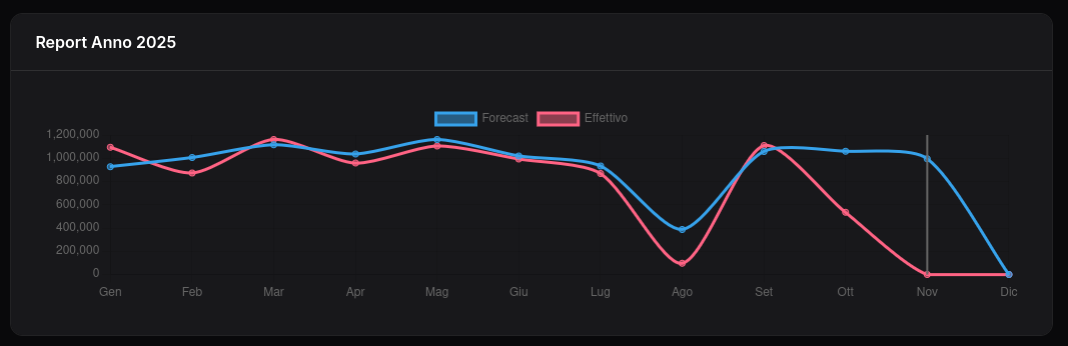
\includegraphics[width=\textwidth]{img/previsione_2025.png}
    \caption{Andamento storico vs previsioni annuali (screenshot della dashboard)}
    \label{fig:forecast-annual}
\end{figure}
\begin{figure}[H]
    \centering
    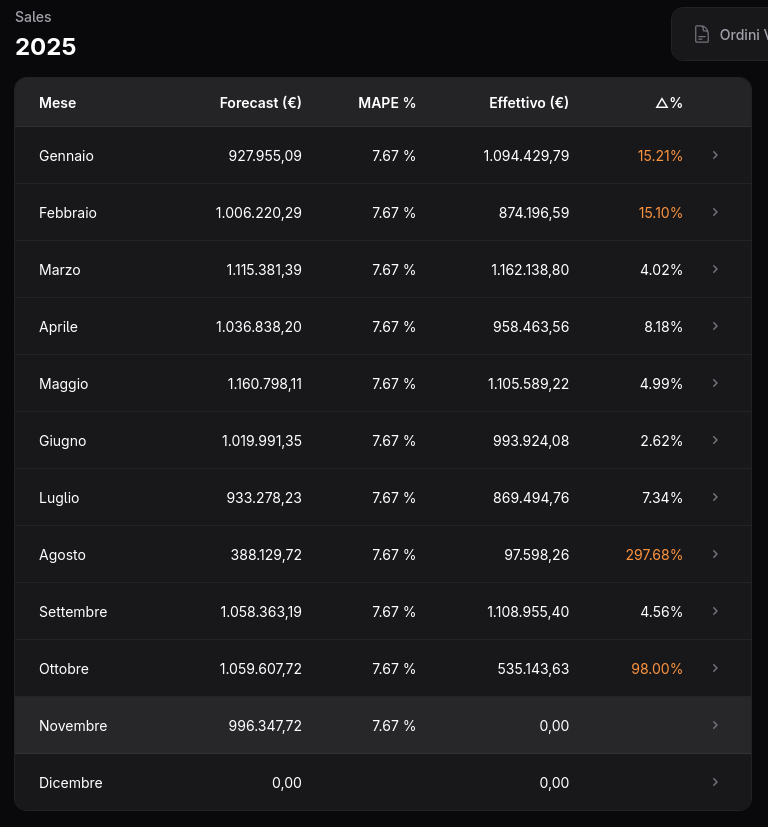
\includegraphics[width=0.9\textwidth]{img/tabella_previsione_2025.png}
    \caption{Tabella di dettaglio delle previsioni annuali}
    \label{fig:forecast-annual-table}
\end{figure}

\subsection{Feature più influenti}
L’analisi SHAP mette in evidenza le variabili che guidano maggiormente le previsioni. Nel grafico, ogni punto rappresenta un campione: i colori indicano il valore della feature (rosso = valore alto, blu = valore basso), mentre la posizione sull’asse orizzontale misura il contributo SHAP (a destra aumenta la previsione, a sinistra la riduce). La densità dei punti lungo l’asse mostra la distribuzione degli impatti.
Alcune delle feature più influenti sono:
\begin{itemize}
    \item \texttt{quantity\_roll\_med6}: media mobile a 6 periodi sulle quantità vendute; valori alti spostano nettamente a destra, segno che volumi recenti elevati trainano la domanda attesa.
    \item \texttt{article\_avg\_monthly\_sale}: media mensile storica per articolo; contribuisce positivamente quando sopra la media, stabilizzando le previsioni su trend consolidati.
    \item \texttt{sales\_history\_ratio}: rapporto tra vendite recenti e storiche; valori alti indicano accelerazione e portano contributi positivi, mentre valori bassi riducono la stima.
    \item \texttt{summer\_shutdown}: flag di chiusura estiva (es. agosto); i punti rossi a sinistra mostrano che quando la chiusura è attiva la previsione cala, come atteso per lo stop produttivo.
\end{itemize}
\begin{figure}[H]
    \centering
    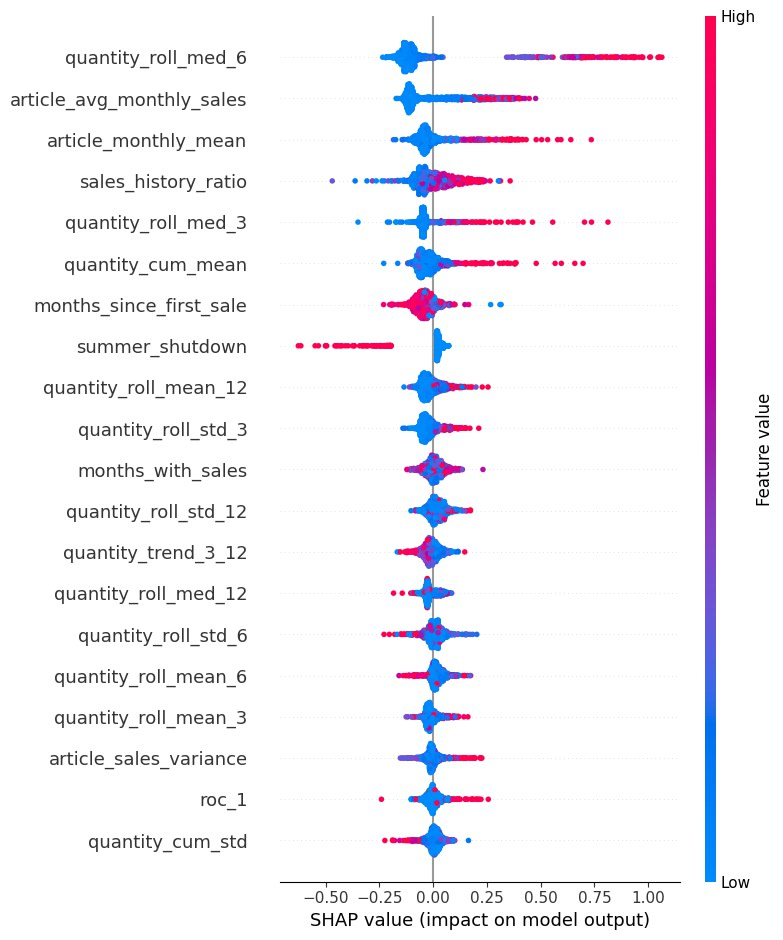
\includegraphics[width=0.95\textwidth]{img/shap_valori.png}
    \caption{Feature più influenti secondo SHAP (valori e segno del contributo)}
    \label{fig:feature-importance}
\end{figure}
\subsection{Miglioramenti futuri}
Nonostante i risultati positivi, ci sono margini di miglioramento per affrontare alcune criticità emerse:
\begin{itemize}
    \item \textbf{Previsioni per singoli articoli}: per quanto l'andamento generale sia buono, le previsioni a livello di singolo articolo mostrano scostamenti più marcati suprattutto per articoli con bassa storicità o stagionalità irregolare. Si prevede di integrare modelli specifici per cluster di articoli simili.
    \item \textbf{Automazione scelta iperparametri}: attualmente l'ottimizzazione degli iperparametri del modello XGBoost è manuale e richiede tempo. L'implementazione di tecniche di AutoML potrebbe velocizzare questo processo e migliorare le performance.
    \item \textbf{Automazione scelta feature}: l'attuale selezione delle feature si basa su analisi statistiche preliminari. L'adozione di metodi automatici di feature selection potrebbe identificare variabili più rilevanti e ridurre il rumore nei dati.
\end{itemize}

\section{Valutazione personale}
Durante lo stage ho avuto l'opportunità di applicare e approfondire diverse competenze tecniche acquisite durante il percorso universitario, in particolare nell'ambito del machine learning, della gestione di progetti software e dell'implementazione di pratiche DevOps come il testing automatizzato e la continuous integration. Ho imparato a lavorare in un contesto professionale, collaborando con un team eterogeneo e affrontando sfide reali legate alla gestione dei dati e alla scalabilità delle soluzioni. 
Questo stage ha rappresentato un'importante esperienza di crescita personale e professionale, che mi ha permesso di consolidare le mie conoscenze e di acquisire nuove competenze utili per il mio futuro lavorativo.

Per quanto riguarda il progetto sviluppato, ritengo che abbia raggiunto gli obiettivi prefissati, fornendo una soluzione efficace per la previsione della domanda e contribuendo al miglioramento dei processi decisionali dell'azienda.
Sono consapevole che ci sono ancora margini di miglioramento e che il progetto potrà evolversi ulteriormente in futuro, ma sono soddisfatto del lavoro svolto e dei risultati ottenuti fino ad ora.

\newpage


    %\backmatter
    % Bibliografia disattivata
    % \input{references/bibliography}
    %\input{references/webliography}
\end{document}
